\documentclass[]{article}
\usepackage{graphicx} % Required for inserting images
\usepackage{amsmath}
\usepackage{amsfonts}
\usepackage{amssymb}
\usepackage{glossaries}
\usepackage{geometry}
\usepackage{appendix}
\usepackage{hyperref}
\usepackage{authblk}
\usepackage{booktabs}

\usepackage{setspace}
\onehalfspacing

\usepackage{biblatex}
\addbibresource{bibliography.bib}

\usepackage{tcolorbox}
\tcbuselibrary{listings,breakable}

\newtcolorbox{notationbox}[1][]{
  colback=blue!3!white,
  colframe=blue!30!black,
  boxrule=0.5pt,
  breakable,
  title=\textbf{Notation},
  fonttitle=\bfseries,
  left=8pt,right=8pt,top=5pt,bottom=5pt,
  #1
}

\newtcolorbox{em_box}[1][]{
  colback=blue!3!white,
  colframe=blue!30!black,
  boxrule=0.5pt,
  breakable,
  title=\textbf{Summary of EM Algorithm},
  fonttitle=\bfseries,
  left=8pt,right=8pt,top=5pt,bottom=5pt,
  #1
}

\usepackage{fancyhdr}
\pagestyle{fancy}
\fancyhead[L]{Bayesian Statistics and Variational Inference}

\begin{document}

\title{Bayesian Statistics and Variational Inference}
\author[]{Hayden Ramm\thanks{hayden.ramm@physics.ox.ac.uk}}

\affil[]{\textit{University of Oxford}}

\date{November 2025}

\maketitle

\begin{abstract}
    The Bayesian paradigm offers us a powerful way of looking at the world. Not does it give us a concrete statistical method for updating our beliefs based on evidence, it also throws open the door to quantifying how well our machine learning models fit our data. However, Bayesian statistics remains widely misunderstood, even within the hard sciences and often to the graduate level. In these notes, I attempt to present a detailed but approachable description of Bayesian statistics. Beyond this introduction, we take a look at Variational Inference, and how Bayes' Theorem allows us to optimize models with unobservable latent variables.
\end{abstract}

\tableofcontents

\section{Preamble}


\subsection{Caveats, Acknowledgements, and Warnings}

These notes were authored in response to how far and thin useful material on the following topics is spread. Different people use wildly different notation to denote the same thing(s), even though we're all talking about the same science. I imagine this reflects the stage at which much of the Machine Learning community is at-- there is a far more limited degree of centralization as compared to, say, particle physics. Often, we all still have to turn to arXiv and GitHub to figure out what's going on.

These notes are not in any way original. They draw extensively from the Stanford CS229 Lecture Notes by Andrew Ng \cite{Ng2023}, the thesis of Yarin Gal \cite{Gal2016}, the review paper by Ankus Ganguly and Samuel Earp \cite{Ganguly2021}, and additional notes from Princeton authored by David Blei \cite{Blei}. My notes here are best seen as a consolidating effort than a novel contribution.

\subsection{A Note on Notation}
In these notes, I try my best to make my mathematics scrutable to the largest audiences. However, in order for the notes to be internally consistent and not confusing, I will (mostly!) refrain from interchanging differing notation, even if that leads me to neglect some notation that is very prevalent in the literature. For the most part, my mathematics should be easily recognisable. 

\begin{notationbox}

$\log(x)$: Logarithms without subscripts are in \textbf{base $e$}, i.e.\ should be read as $\log_e (x)$.
\\\\
$P(A,B)=P(A\cap B)$: \textbf{Probability of $A$ \textbf{and} $B$}. These two ways of writing it are equivalent. I will very occasionally swap between the two depending on which point I want to illustrate, but will mostly stick to the $(A,B)$ notation.
\\\\
$p(x;\theta)$: A probability density function ($p$) of a random variable ($x$) parametrized by some $\theta$.
\\\\
$\mathbb{E}_{x \sim p(x)}\left[f(x)\right]$: The \textbf{expectation value}, with respect to some random variable (r.v.) $x$, of some function of $x$, $f(x)$. In the notes of others, they may simply write $\mathbb{E}_x \left[f(x)\right]$ or even $\mathbb{E}_{p(x)} \left[f(x)\right]$ to denote the same thing.
\\\\
$(\Omega, \mathcal{F}, \mathbb{P})$: A \textbf{probability space}, which is defined by: $\Omega$, a \textbf{sample space}; $\mathcal{F}$, an \textbf{event space}; and $\mathbb{P}$, a \textbf{probability function}. I point the interested reader to ref.~\cite{Weber2014} for more details.
\\\\
$\mathcal{D}=\{ x^{(i)}, y^{(i)} \}_{i=1}^N$: Denotes some \textbf{dataset} (on which we train a neural network). This includes both input features ($x^{(i)}$) as well as the labels ($y^{(i)}$). The subscript and superscript on the right hand side of the curly braces are there to denote that we have a dataset of $N$ different data points, and that we label them with an index $i$, which runs from $1$ to $N$
\\\\
$\theta$: The \textbf{parameters of a machine learning model}. We often think of this as a (column) vector, where each of the entries of the vector is a different parameter of the model. These parameters are the model's weights $w$ and biases $b$.

\end{notationbox}


\section{Introduction}
We begin our exploration of Bayesian Statistics by considering the conflicting points of view of two fictitious statisticians as they try to estimate the probability, $p$, of observing heads during a \textit{biased} coin toss. See which viewpoint you agree with more.

\textbf{Frequentist}: ``The probability of landing heads on a coin toss, $p$, is unknown, but fixed.''

\textbf{Bayesian}: ``The probability of landing heads on the coin toss, $p$, is some random variable with its own distribution. Nature herself doesn't even know what it is.''


In many ways, the Bayesian viewpoint is the more conservative, if perhaps less intellectually satisfying. Surely our lack of knowledge when it comes to the value of $p$ is a shortcoming of ours, not a shortcoming of the nature's. Surely there is a ``right answer'', a ``true value''!

Many people conceive of probability like this. To say that one view is correct and the other is incorrect is a philosophical, not mathematical, debate. However, the Bayesian framework has its place, too; it gives us a powerful framework for adjusting our beliefs about the world as some new evidence arises. Even better, it allows us, at least in theory, to calculate some probability distribution about observables of interest, here the probability of getting heads in a biased coin toss, rather than forcing us to converge to some fixed estimate. Even if the chance of getting heads is one in a million, it is still theoretically possible to observe a million heads in a row. The probability of this just happens to be vanishingly small. That doesn't make it zero.

We also know from our studies of quantum mechanics, and subsequently quantum field theory, that the world is highly non-deterministic. You can't predict the future with $100\%$ certainty. Nothing is ``knowable'' in the absolute, classical sense, but there are plenty of things which are ``estimable''.

In machine learning, the Bayesian framework helps us in quantifying the quality of our model. How well do our parameters describe the data? How much do we trust the model? How do we adjust the model based on the data we have? And so on.

\section{Bayesian Statistics}

\subsection{Conditional Probability}
In many cases, we are interested in the probability of some event $A$ given that some other event, $B$, has already occurred. For example, let $A$ and $B$ denote some meal-related events, i.e. $A=\text{Had an Early Dinner}$, and $B=\text{Had a Late Lunch}$. We can see that we'd expect the chances of us having an Early Dinner to be influenced by whether we had a Late Lunch. In other words $P(A) \neq P(A|B)$, where we have introduced the pipe symbol $|$ to denote conditions on $A$; we read $P(A|B)$ as ``the probability of $A$ given that $B$ has happened''.

We motivate this notation by taking a closer look at what $P(A)$ actually means. We can rewrite $P(A)$ as $P(A|\text{All possible universes})=P(A|\Omega)$, where ``all possible universes'' ($\Omega$) means all possible outcomes, i.e.\ defines a \textbf{sample space}. 

$\Omega$ includes every possible outcome: a universe in which it rained, the universe where it rained and then we had a bagel, the universe in which it didn't rain but we did have a bagel... We know that $P(\text{All possible universes})=P(\Omega)=1$; if it were equal to less than $1$, we cannot have accounted for all possible outcomes. The probabilities of all possible outcomes \textit{must sum to exactly one}.

The probability of $A|B$ is given by:
\begin{equation}\label{equation:conditional_prob}
    P(A|B) = P(A \cap B)/P(B) \equiv P(A,B)/P(B)
\end{equation}
We can visualize this graphically (fig. \ref{fig:conditional_prob_venn}) and explain it heuristically as follows: to calculate $P(A|B)$, we can \textit{only} take into account universes where $B$ has happened. We want to calculate the probability of $A$ given that $B$ has happened. The only part of the Venn Diagram in fig. \ref{fig:conditional_prob_venn} in which $A$ can happen (given that $B$ has happened) is in the overlap, $A\cap B$. Equation \ref{equation:conditional_prob} tells us that $P(A|B)$ is given by the fraction of ``$B$-has-happened universes'' in which $A$ also occurs.

\begin{figure}
    \centering
    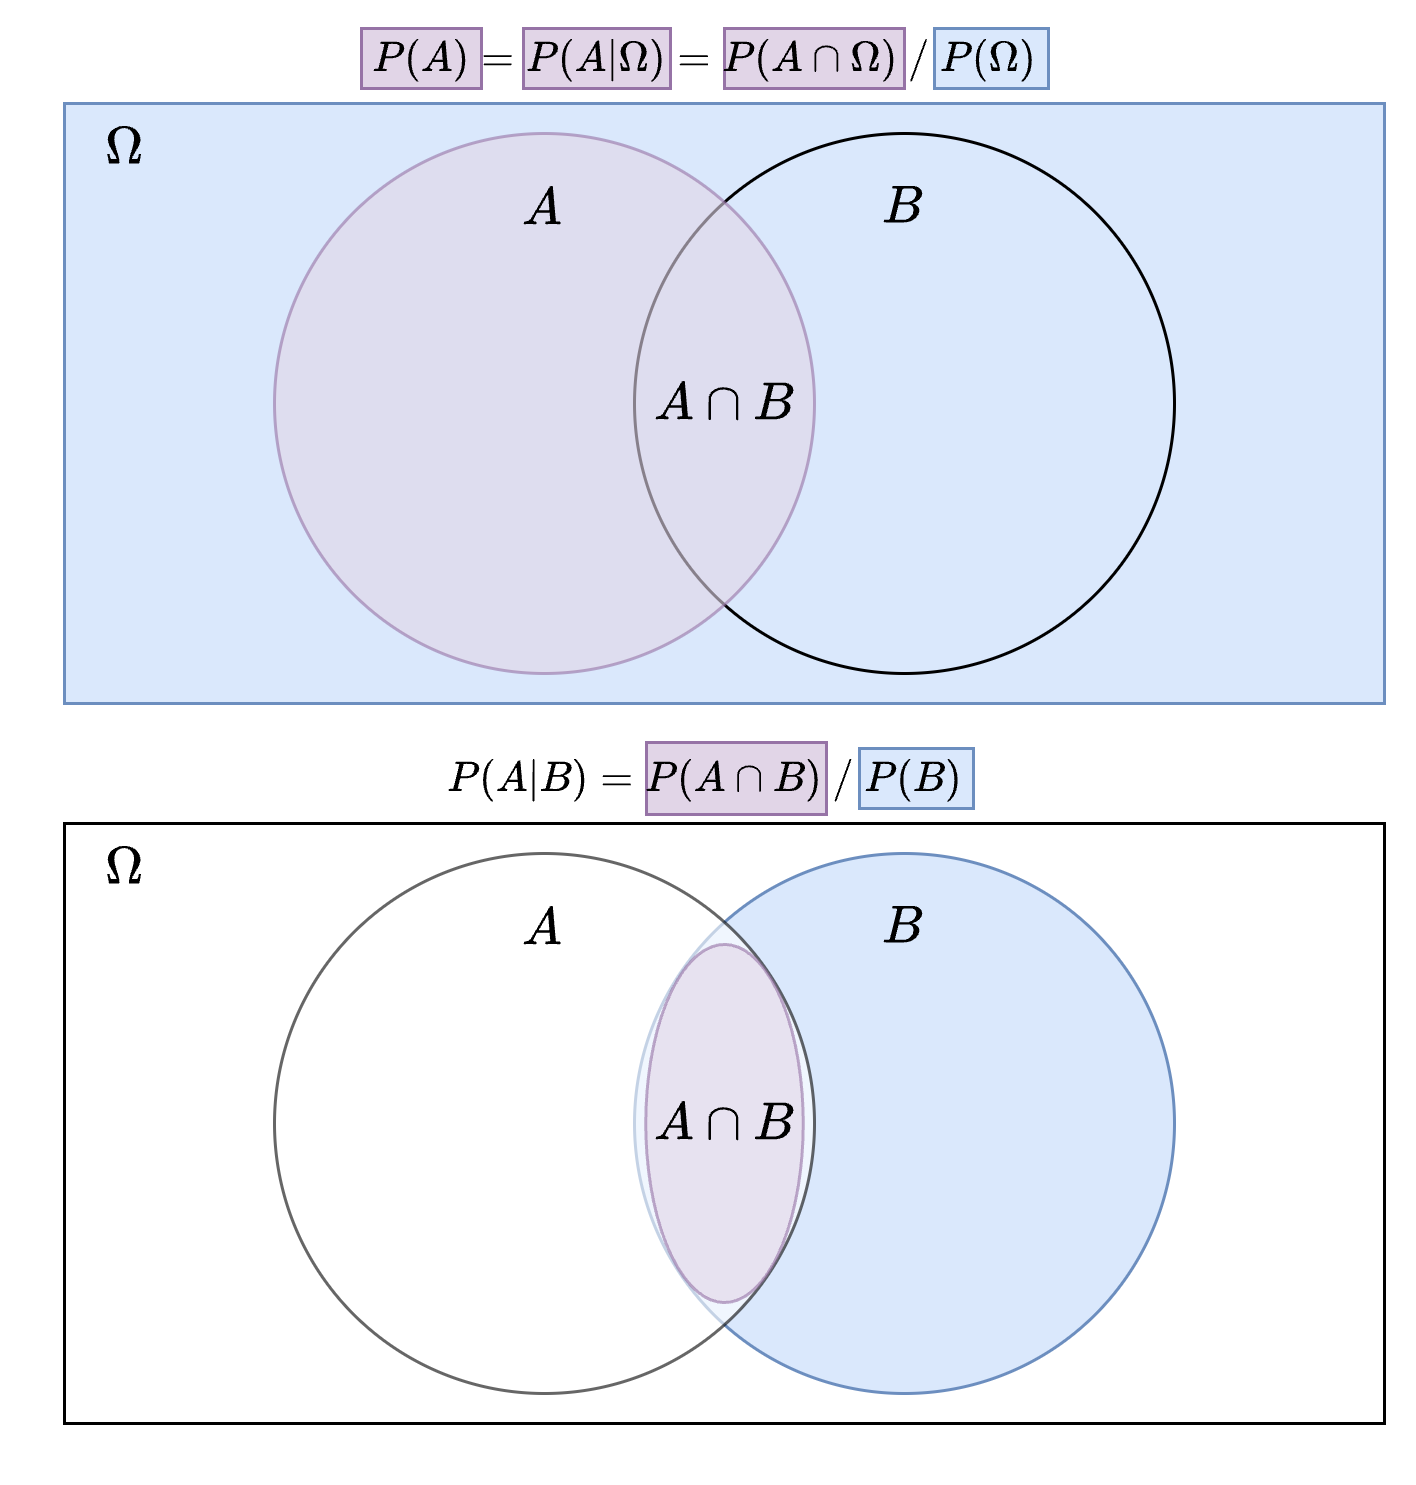
\includegraphics[width=0.5\linewidth]{Figures/conditional_prob.png}
    \caption{Demonstration of conditional probability. In the first case, $P(A)$, our denominator is given by $P(\Omega)=1$; we are restricted to $\Omega$, which represents ``all possible universes'' (all possible outcomes), thus we are \textit{unrestricted}. In the second case, $P(A|B)$, our denominator is given by $P(B)$, i.e. we have been restricted only to the universes in which $B$ has occurred.}
    \label{fig:conditional_prob_venn}
\end{figure}

\subsection{The Law of Total Probability}\label{section:total_prob}
Now that we have developed both the notation and a conceptual understanding of conditional probability, we turn to an important result in probability: the \textbf{Law of Total Probability}. Here is the statement of the Law in the case of \textbf{discrete} random variables:
\begin{equation}
    P(A) = \sum_i P(A|B_i)P(B_i)
\end{equation}

And in the continuous case, where $A$ and $B$ are continuous random variables instead of discrete ones, we rewrite this as an integral:
\begin{equation}\label{eq:total_prob_cont}
    P(A) = \int \text{d}B~P(A|B)P(B)
\end{equation}

We can see how this Law makes sense with a simple example. Let's say that $A$ is the probability that we watched TV yesterday. $B$ is the probability that it was sunny yesterday. Let's make the simplifying assumption that there are only \textit{two} possible outcomes for the weather: sun and no sun. This means that $B_i=\text{Sun}$ or $B_i=\text{No Sun}$. Therefore, we have:
\begin{equation}
    P(\text{Watched TV}) = P(\text{Watched TV}|\text{No Sun)}P(\text{No  Sun}) + P(\text{Watched TV}|\text{Sun})P(\text{Sun})
\end{equation}
If we then expand our universe to include other possible weather conditions, we would simply just introduce more terms to the sum above.

We can say that we have ``marginalized'' over $B$, i.e. by accounting for all possible outcomes of the random variable $B$, we have removed it from the picture. In our case we can think of this as ``we accounted for the chance of us watching TV, \textit{regardless} of the weather. We considered every possible condition of the weather, calculated the probability of watching TV in each case, and then summed up those probabilities. Weather is no longer an object, as we've accounted for every possible weather condition.'' 

Therefore, what we are left with must be the probability of watching TV \textbf{no matter the weather}.

\subsection{Bayesian Statistics}

Bayesian statistics, in particular Bayes' theorem, helps us to quantify why, \textit{in general},
\begin{equation}\label{eq:a_b_not_b_a}
    P(B|A) \ne P(A|B)
\end{equation}
We will shortly explore the case in which this equality does happen to hold, but those cases should be considered the exception to the rule rather than the rule.

Indeed, there is every reason to suppose equation \ref{eq:a_b_not_b_a} is true. Let's imagine we are concerned with calculating two probabilities: the first is $P(\text{We go inside} | \text{It rains})$. This, of course, should be different from $P(\text{It rains}|\text{We go inside})$. This is because, in the latter case, there are all kinds of scenarios in which we choose to go inside even if it isn't raining (dinner is ready, a football game is on...) So, though we may choose to go inside $99\%$ of the time that it rains, i.e. $P(\text{We go inside}|\text{It rains}) = 0.99$, we would expect $P(\text{It rains}|\text{We go inside})$ to be much lower: just because we went inside doesn't mean that it rained. Maybe we went inside to eat, even though it was sunny.

\subsubsection{Bayes' Theorem}

Bayes' Theorem, powerful though it may be, is nothing more exciting or exotic than the statement that $P(A \cap B) = P(B \cap A)$, which we take as axiomatic. We can proceed as follows:
\begin{equation}
    P(A \cap B) = P(A|B)P(B)\\
\end{equation}
\begin{equation}
    P(B \cap A) = P(B|A)P(A)
\end{equation}
therefore, using $P(A \cap B) = P(B \cap A)$,
\begin{equation}
    P(A|B)P(B) = P(B|A)P(A)
\end{equation}
\begin{equation}\label{eqn:bayes_theorem}
    P(A|B) = \frac{P(B|A)P(A)}{P(B)}
\end{equation}
and this is the statement of \textbf{Bayes' Theorem}.

We can immediately note that, in the \textit{particular case} that $P(A)=P(B)$, we recover from Bayes' Theorem that $P(A|B) = P(B|A)$, but this will not hold in general. In our example above, this means that if the probability of us going inside (for any reason) is equal to the probability of it raining, then $P(\text{We go inside} | \text{It rains}) = P(\text{It rains}|\text{We go inside})$. 

This makes intuitive sense: given two random events with identical probability, (1) it rains and (2) we go inside, we expect them to be on equal footing, i.e. if we labeled $A=\text{It rains}$ and $B=\text{We go inside}$, exchanging the labels $A \leftrightarrow B$ shouldn't result in any meaningful change to the mathematics. However, if they do \textit{not} have equal probabilities, we of course would expect the change $A \leftrightarrow B$ to be meaningful and non-trivial.

\subsubsection{Pieces of the Bayesian Pie}

Let's restate Bayes' Theorem in a more insightful form:

\begin{equation}
    P(A|B) = \frac{P(B|A)P(A)}{\int \text{d}A'~P(B|A')P(A')}
\end{equation}
which looks intimidating but is in fact trivial. Let's focus on the \textit{denominator}, which is typically given the name \textbf{marginal likelihood} or \textbf{evidence}. We have used a simple result, the \textbf{Law of Total Probability} for \textbf{continuous variables} (recall equation \ref{eq:total_prob_cont}), to rewrite $P(B)$ as $\int \text{d}A'~P(B|A')P(A')$, where we have assumed that the variables are continuous rather than discrete (hence the integral rather than a sum). Note the presence of the word ``marginal''-- this refers to the fact that we are summing over all possible values of a random variable, $A$, i.e. ``marginalizing'' over it, as we discussed in Section \ref{section:total_prob}. The prime notation, $A'$, is there to emphasize that $A$ is a dummy variable in the denominator, whereas it is \textit{not} a dummy variable in the numerator. In the numerator, $A$ takes a particular value; in the denominator, we sum over \textit{all possible values} of $A$.

Now, we take a look at the numerator: we refer to $P(B|A)$ as the \textbf{likelihood}, and $P(A)$ as the \textbf{prior} probability (or simply the ``prior''). Both of these labels will make more sense once we turn to the use of Bayes in machine learning (Subsection \ref{subsubsection:bayes_ML}).

Finally, we turn to the left hand side: $P(A|B)$ is referred to as the \textbf{posterior} probability (or just ``posterior''). This distinguishes it from the \textbf{prior}, $P(A)$; in the case of the ``posterior'', we have in some sense ``updated'' our distribution for $A$ given some new information. In this case, the ``new information'' is the value taken by $B$. So, our \textbf{prior} distribution encodes our belief about $A$ before any new information, and our \textbf{posterior} distribution encodes our belief about $A$ after we observe $B$. The implications of ``updating'' beliefs is once again clearer in the context of updating a machine learning model during training.

\subsubsection{Librarians and Farmers}

As an illustrative example of Bayes' Theorem (and its consequences), we will turn to the classic ``farmer or librarian'' problem made famous by everyone from Grant Sanderson \cite{SandersonBayes2016} to Daniel Kahneman \cite{kahneman2011thinking}. We will repeat it here because it's fun, and memorable.

We are given a description of an individual\footnote{This is my own personal distillation of the problem statement; you will find different ones.}:

``There are only two jobs in this town: farming and librarians. There are twenty times as many farmers as librarians. X, a worker in the town, is very shy and bookish. She prefers reading to socializing. Is X more likely to be a librarian, or a farmer?''

Additional information: $40\%$ of librarians are bookish. $10\%$ of farmers are bookish.

Most people, at first glance, answer \textit{librarian}: ``Of course,'' they say. ``Librarians must be at least a little bookish! Who cares that there are more farmers?'' Notice the subtle error in this reasoning: this answer \textbf{assumes we are asking for} $P(\text{Bookish}|\text{Librarian})$. We are not!! What the question above is actually asking for is a value for $P(\text{Librarian}|\text{Bookish})$. Most people substitute this for the easier estimate, $P(B|L)$, and (to be fair to them) this is normal (we have shortened ``librarian'' to L and ``bookish'' to B).

The correct answer is, famously, \textit{farmer}. This isn't because any individual farmer is more likely to be bookish than any individual librarian: it's because there are \textbf{so many more farmers than librarians} in our example. As a result, even if a small fraction of farmers are bookish, there can still be more bookish farmers than there are bookish librarians if the population of farmers swamps that of librarians. We illustrate this graphically in figure \ref{fig:farmers_librarians}, and mathematically below.

Recall Bayes' Theorem:
\begin{equation} \label{eq:bayes_librarians}
    P(L|B) = \frac{P(B|L)P(L)}{P(B)} = \frac{P(B|L)P(L)}{P(B|L)P(L) + P(B|F)P(F)}
\end{equation}
where we have expanded the denominator using the Law of Total Probability (section \ref{section:total_prob}), remembering that we have assumed people can only be either farmers or librarians. Our problem statement tells us that there are twenty times as many farmers as librarians, i.e. for every $21$ people, only $1$ is a librarian. Hence:

\begin{align}
    &P(F) = 20/21\\
    &P(L) = 1/21
\end{align}

We have already been supplied with $P(B|L)=0.4$ and $P(B|F)=0.1$. We plug these into equation \ref{eq:bayes_librarians} and recover:

\begin{equation}
    P(L|B) = \frac{0.4\times1/21}{0.4\times1/21 + 0.1\times20/21} = 1/6
\end{equation}

i.e. there is only a $1$ in $6$ chance of the anonymous individual being a librarian! This shows us that $P(F|B) > P(L|B)$ even though $P(B|F)<P(B|L)$ for our population.

This is a particular case of the \textbf{base rate fallacy}; we have focused on specific details (our prior beliefs about the bookish-ness of farmers and librarians) and neglected key statistical factors, namely the \textbf{prevalence of farmers and librarians in the population}. 

\begin{figure}
    \centering
    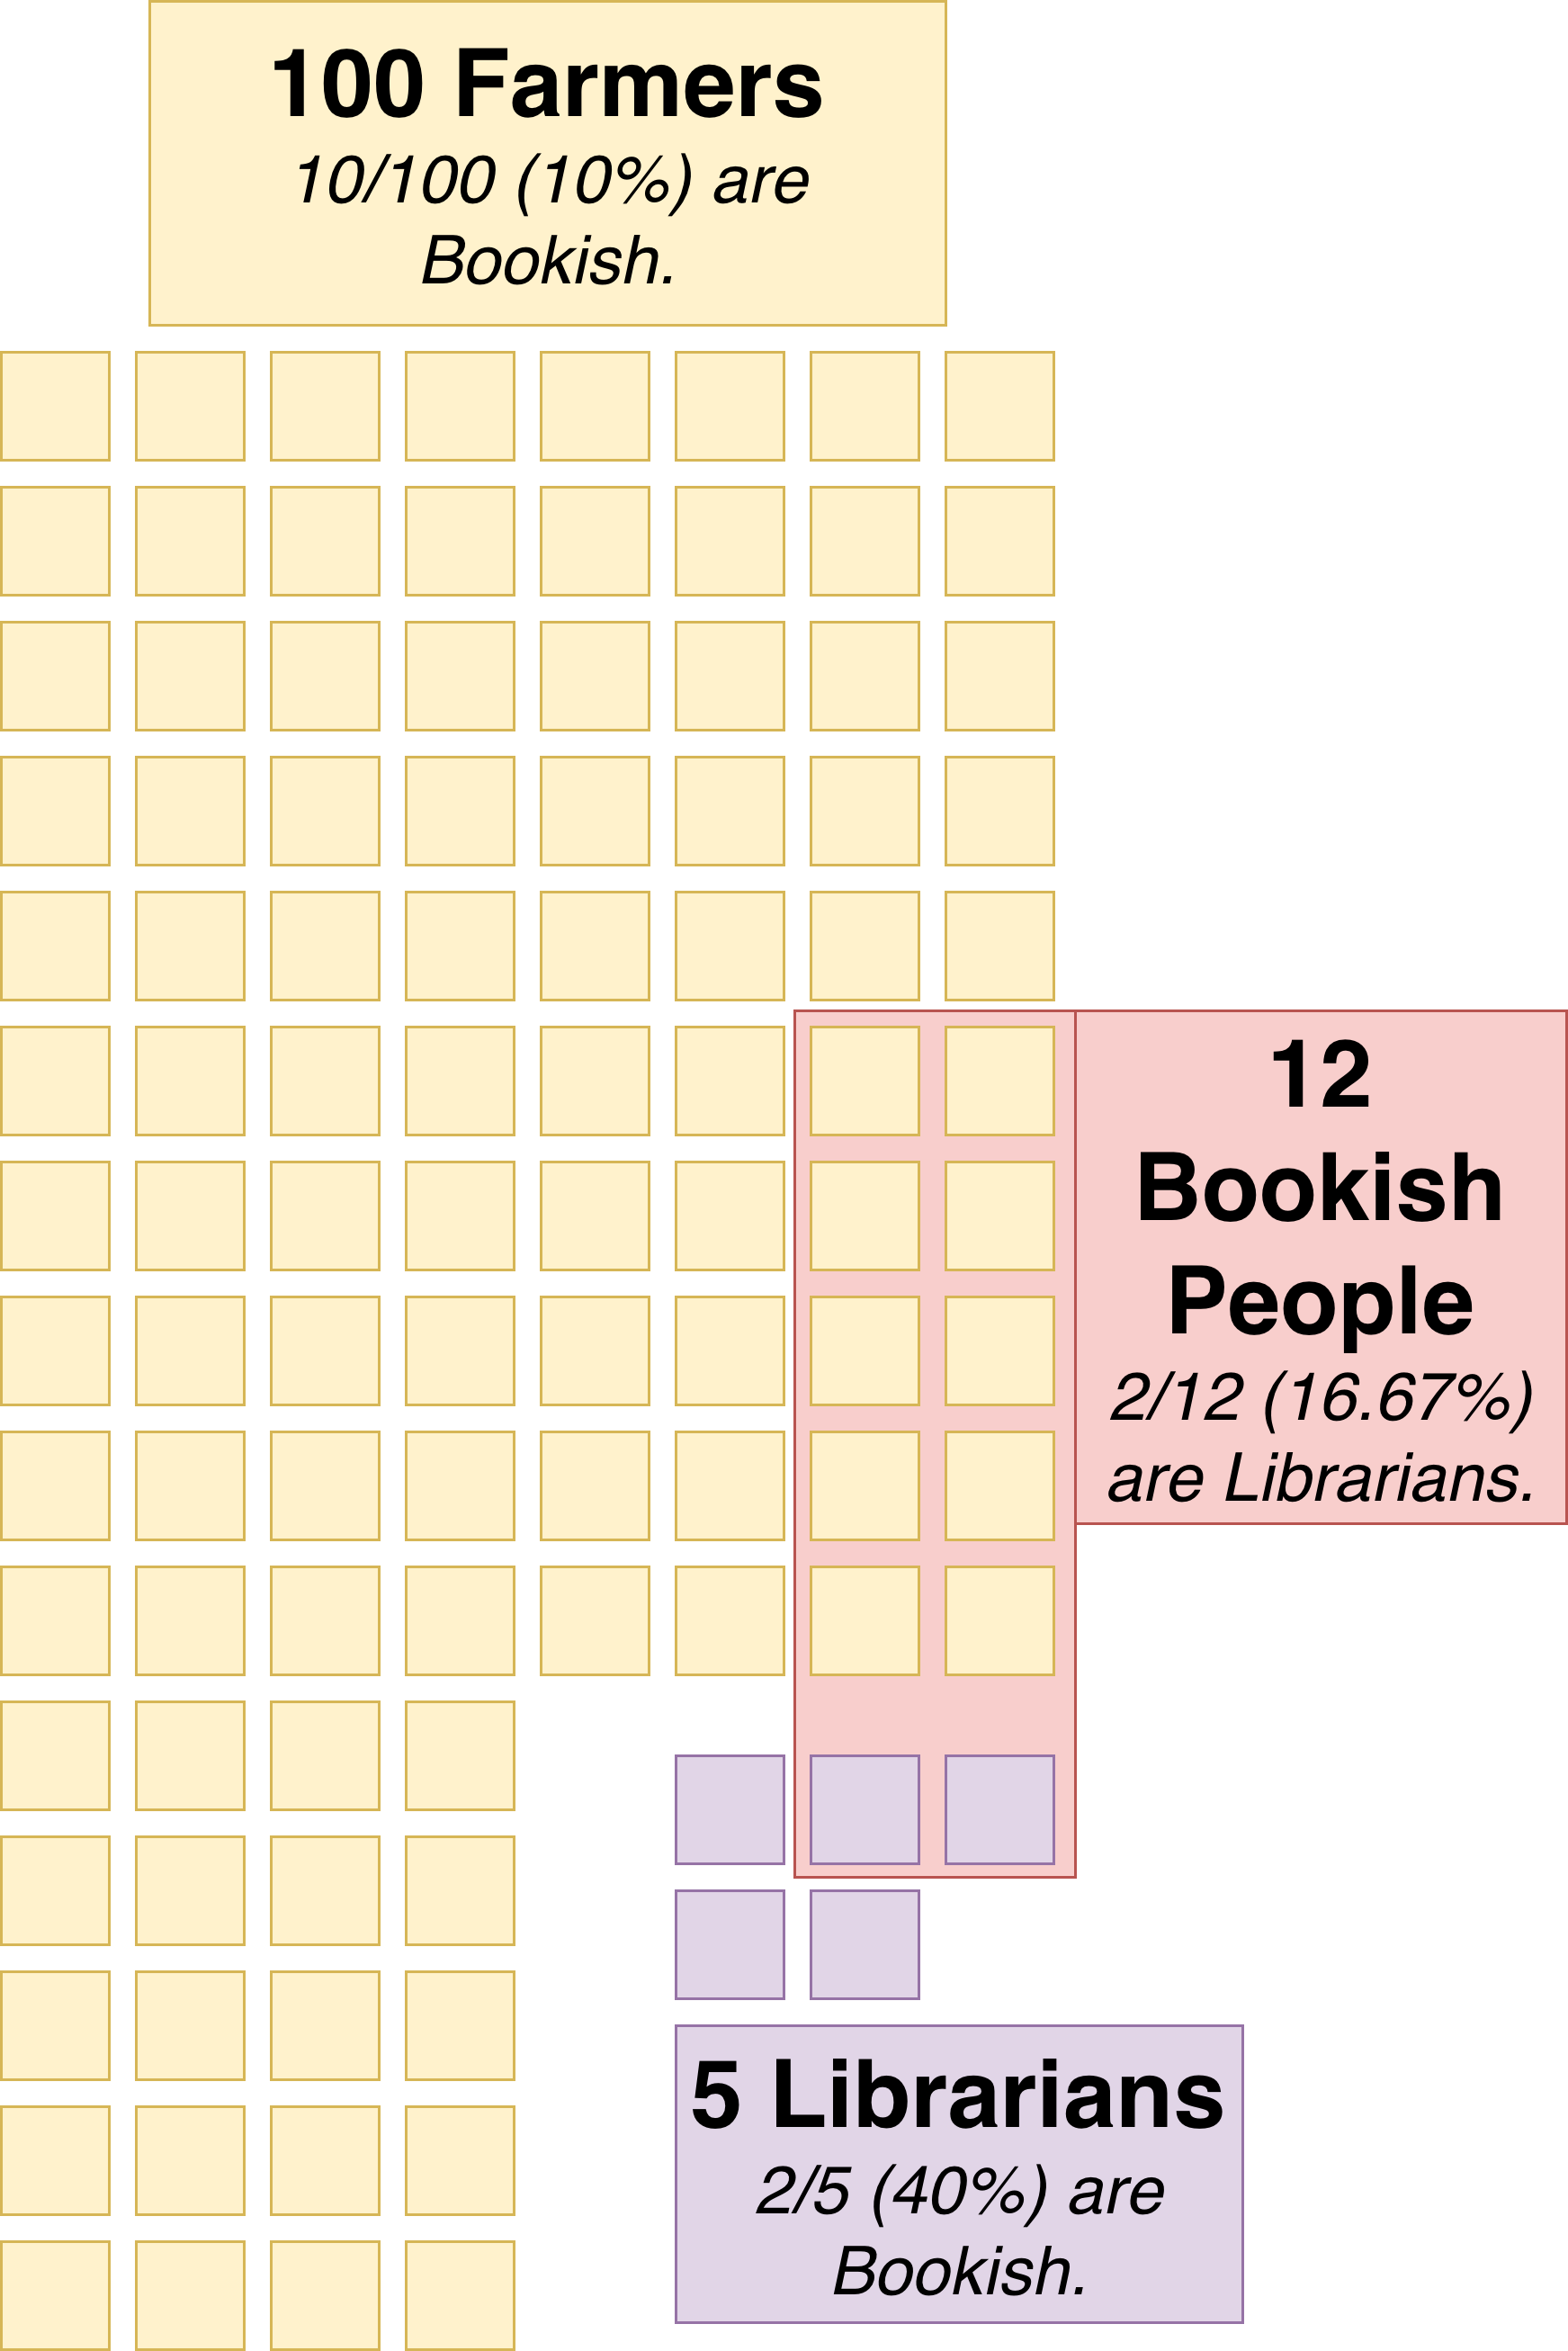
\includegraphics[width=0.35\linewidth]{Figures/farmers_librarians.png}
    \caption{Illustration of how Farmers outnumber Librarians in the ``Bookish'' category, even though individual Librarians are more likely to be Bookish than individual Farmers.}
    \label{fig:farmers_librarians}
\end{figure}

\subsubsection{Bayes in Machine Learning}\label{subsubsection:bayes_ML}
Let's reexamine Bayes' Theorem in the context of machine learning. To set the stage, we focus on the following quantity: $P(\theta | \mathcal{D})$. This will be our \textbf{posterior}. We can think of this as ``how realistic are our model's parameters given we've just observed some data, $\mathcal{D}$?''. In an ideal world, we would maximize this value; this is the process of choosing the most ``believable'' parameters given some data. If we observe a bunch of data $\mathcal{D}$ with some mean $\mu=20$, we may start to be skeptical of a model (say, with parameters $\theta_1$) that predicts a mean of $\hat\mu = 1$. This ``skepticism'' means that our value of  $P(\theta=\theta_1 | \mathcal{D})$ is low. Note that we could actually still be right in estimating the mean at $1$-- perhaps we just got unlucky and picked a bunch of outliers in a row.

Now, we have an intuitive understanding of what a \textbf{posterior} is; given (new) data $\mathcal{D}$, we update our beliefs about our model parameters $\theta$. Do our parameters still look reasonable after we look at the data? We use Bayes' Theorem (eq. \ref{eqn:bayes_theorem}) to express this posterior distribution for the model parameters, $\theta$:
\begin{equation}\label{eqn:bayes_theorem_model_likelihood}
    P(\theta | \mathcal{D}) = \frac{P(\mathcal{D} | \theta) P(\theta)}{\int \text{d}\theta'~ P(\mathcal{D} | \theta') P(\theta')}
\end{equation}

We often cannot calculate this quantity directly as the integration in the denominator, the \textbf{marginal likelihood}, is almost always intractable; we would have to integrate over \textit{the entire parameter space} for $\theta$, that is, every possible value of every single parameter. Even in modest models, this is infeasible. This is what leads us to make the \textbf{maximum likelihood estimation}, or \textbf{MLE}. In this case, we maximize the likelihood directly instead of the posterior, as we notice that the posterior is proportional to the likelihood: $P(\theta | \mathcal{D}) \propto P(\mathcal{D} |\theta) P(\theta)$ (as per eq. \ref{eqn:bayes_theorem_model_likelihood}). In the MLE, we choose our ``ideal'' model parameters, $\theta^*$, as being
\begin{equation}
    \theta^* = \arg\max_\theta ~ P(\mathcal{D} | \theta)
\end{equation}
This means that, in the MLE, we select our $\theta$ as to maximize the likelihood, as estimated by our model, of observing the given dataset $\mathcal{D}$. This is a reasonable assumption, and this calculation is tractable; our model(s) will output this value for us, and so we are now limited by computational power and the size of our model.

\section{Variational Inference}

\subsection{What is Variational Inference, and Why Do It?}

\subsubsection{Inference in Machine Learning}

Once we have trained a model on a dataset, $\mathcal{D}$, we ideally want to use it to generate new predictions on unseen data. An example of deploying a model on unseen data is when we apply it to a \textbf{test dataset}, which is a dataset which we use to quantify model accuracy and/or performance without adjusting its parameters. If our model tests well on unseen data, therefore demonstrating its ability to \textbf{generalize}, we next need to go about deploying it in the real world.

$\mathcal{D}$ can also include, as a subset, a \textbf{validation set}. We adjust the model using both the training set (via gradient descent) and validation set (e.g. by adjusting parameter number, depth, width, etc.)\footnote{In cross-validation, the partition between training and validation sets changes, in which case we will end up using gradient descent on the entirety of $\mathcal{D}$.}. However, in both cases, the model has been optimized to fit the training and validation data.

We now try to produce a model prediction for an unseen piece of data, $\textbf{x}^*$. We define the model \textbf{inference} as follows:
\begin{equation}\label{eq:inference}
    p(y^* |\textbf{x}^*, \mathcal{D};\theta) = \int \text{d}z~p(y^*|\textbf{x}^*, z;\theta)p(z|\mathcal{D};\theta)
\end{equation}
where we add the subscript $\theta$ to show explicitly that our model is parametrized by a set of weights and biases, $\theta$. We have also introduced $z$ to denote \textbf{latent variables}, which is an umbrella term for variables that are not observed directly but instead ``inferred'' at training time. Some examples are as follows:
\begin{itemize}
    \item In a Mixture of Gaussians (MoG) model, the ``class labels'' denoting different Gaussians are an example of latent variables (fig. \ref{fig:mixture-of-gaussians}).
\end{itemize}

We immediately run into serious problems because we don't have access to these variables directly-- we will address this in Section \ref{section:expectation_maximization}. Furthermore, the posterior distribution, $P(z|\mathcal{D} ;\theta)$, is intractable. We will address this in Section \ref{section:estimating_p|z}.

You will notice we have explicitly shown that the posterior $P(z|\mathcal{D};\theta)$ is parametrized by $\theta$; calculating the likelihood of the model's latent variables based on the data is necessarily a function of the model's parameters.

\subsubsection{Mission Statement}
We almost always find it intractable (impossible) to compute a posterior distribution due to the integral which appears in the denominator (recall that this is also called the \textbf{evidence} or \textbf{marginal likelihood}).

This is particularly problematic if we would like to run \textbf{inference} (recall equation \ref{eq:inference}) for a model with some hidden or \textbf{latent} variables, which we will talk about a bit more in the next Section (\ref{section:latent_variables}).

Wouldn't it be nice if we could somehow approximate a posterior distribution, $p(z|\mathcal{D})$, using some function, $q$, such that:
\begin{equation}
    p(z | \mathcal{{D}};\theta) \approx q_\nu(z)    
\end{equation}
where we are interested in updating our beliefs about some variables, $z$, given observations of some dataset, $\mathcal{D}$? $q(z)$ is our approximation for the posterior, which would otherwise involve a possibly intractable integral.

We rewrite $q(z) = q_\nu(z)$ to allow some \textbf{variational parameters}, $\nu$. We can tweak these parameters, $\nu$, until our approximating distribution, $q_\nu (z)$, approximates the posterior as closely as possible. We choose $q_\nu (z)$ from some \textbf{family of distributions} such that both $q_\nu (z)$ itself, and expectation values calculated from it, are \textbf{tractable} (otherwise there's no point).

The term \textbf{variational inference} refers to our attempts to perform the intractable inference calculation (equation \ref{eq:inference}) with the following approximation: 

\begin{equation}\label{eq:approx_inference}
    p (y^{*} | \textbf{x}^*, \mathcal{D};\theta) \approx \int \text{d}z~ p (y^*|\textbf{x}^*, z;\theta)q_\nu (z) 
\end{equation}

Finding a good $q_\nu$ to approximate equation \ref{eq:approx_inference} is the aim of \textbf{variational inference}.

\subsubsection{A Note on Latent Variables and Model Parameters}\label{section:latent_variables}
In Yarin Gal's thesis \cite{Gal2016} (from which I learned much of what I know about variational inference), as well as in other works focusing on Bayesian networks, the distinction between \textbf{latent variables} and \textbf{model parameters} can become fuzzy. In Bayesian networks, there is a posterior over the model parameters themselves, and so are in some sense treated as ``unobserved'', or \textbf{latent}. Gal explicitly treats the model parameters as the latent variables, which he denotes as $\boldsymbol{\omega}$. Here I will keep the distinction between model parameters and latent variables in general explicit.

\begin{figure}
    \centering
    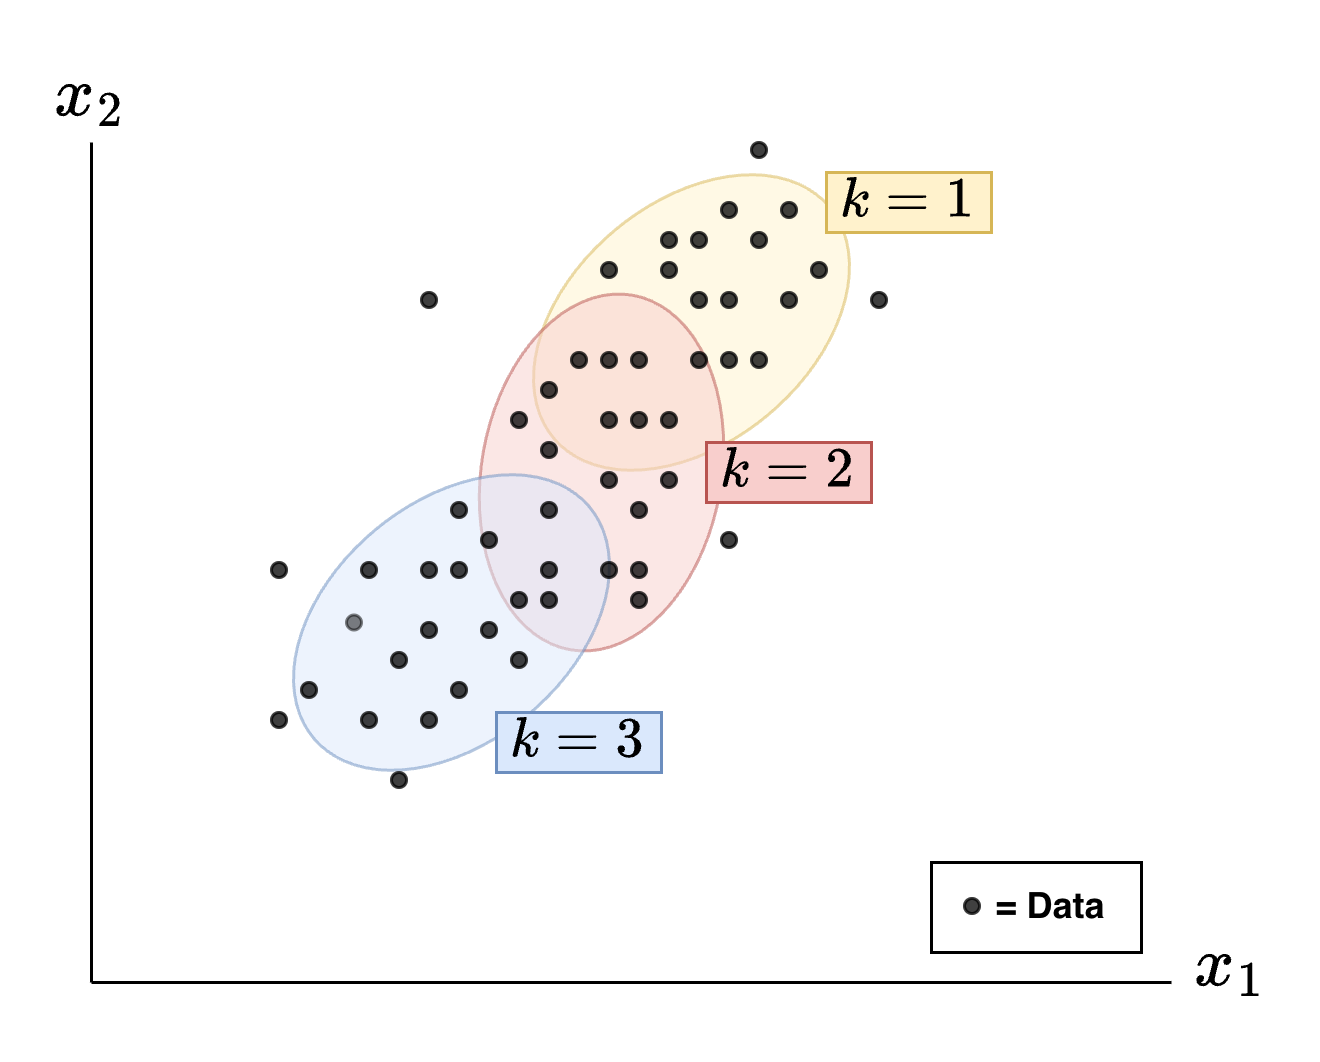
\includegraphics[width=0.5\linewidth]{Figures/mixture_of_gaussians.png}
    \caption{Fictitious Mixture of Gaussians (MoG) model. We fit a distribution to the data by superimposing three different Gaussians, shown in yellow, red, and blue; we can label each of these three Gaussians with a ``class label'', $k$. The value of these class labels are not directly observed during the training process, and are examples of ``latent variables''.}
    \label{fig:mixture-of-gaussians}
\end{figure}

\subsection{Entropy and Information}\label{section:entropy_and_information}

Very shortly, we will introduce an important quantity called the \textbf{KL Divergence} in Section \ref{section:kl_divergence}. This is usually quoted without much quantitative motivation, and it is precisely this type of motivation I will try to provide here.

First, let's define the \textbf{surprisal}, or \textbf{self-information} of an event. The surprisal gets its name from the fact that it quantifies how ``surprising'' an event is. If an event is very unlikely, i.e. ``surprising'', it carries with it a lot of \textbf{information}. 

Reporting the occurrence of events with a high probability contains little information. Therefore, ``unsurprising'' events are in a sense ``low-information'' events. We denote self-information of an event $E$ as $I(E)$.
\begin{align}\label{eq:self-information}
    &I(E) \text{[nats]} = \log \frac{1}{P(E)} = -\log P(E)
    \\
    &I(E) \text{[bits]} = \log_2 \frac{1}{P(E)} = -\log_2 P(E)
\end{align}
where the unit of self-information in equation \ref{eq:self-information} is the \textbf{nat}. If we define self-information as $-\log_2 P(E)$, then the units are the Shannon (\textbf{Sh}), and hence $1$ bit = $\log 2$ nats.

Let us now define the \textbf{Shannon entropy} (also called \textbf{information entropy}) as follows:
\begin{equation}\label{eq:shannon_entropy}
    \mathbb{H}(X) := -\sum_{x \in X} P(x) \log P(x) = -\mathbb{E}_{x\sim P(x)}[\log P(x)]
\end{equation}
Physicists like myself should immediately recognize the direct analogy to \textbf{Gibbs entropy} in thermodynamics. 

We can interpret the Shannon entropy by considering a biased coin toss. We have two outcomes: heads ($H$), or tails ($T$), i.e. $X=\{H, T\}$. Let the probability of getting heads be defined as $P(H)=p$. Therefore, we write the Shannon entropy for the coin toss as
\begin{equation}\label{eq:shannon_entropy_coin_toss}
    \mathbb{H}(X) =-P(H) \log P(H) -P(T) \log P(T) = -p \log p - (1-p) \log (1-p)
\end{equation}
Let's consider two cases. 

\begin{align}
    (a)~&p=0.5: \mathbb{H}(X) = -0.5 \log 0.5 - 0.5 \times \log 0.5 &&= \log 2\\
    (b)~&p=0.0: \mathbb{H}(X) = -0\times \log 0 - 1 \times \log1 &&= 0 
\end{align}

We immediately notice that entropy is $0$ when one outcome is certain, and entropy is large (in fact, is \textbf{maximized}) when the two outcomes have equal probability. This is illustrated in figure \ref{fig:entropy_cointoss}. If one outcome is certain, we have no ``freedom of choice''; there is nothing we can do to change the outcome, and so no information can ever be conveyed by the outcome of the coin toss. We already know the outcome with certainty, and observing that outcome will not enhance our knowledge of the system. We can never be ``surprised'', and if we can't be surprised, we can't learn anything.

Note that if we had six outcomes of equal probability, for example in the case of a fair six-sided die, the entropy would be $6 \times -\frac{1}{6} \log \frac{1}{6} = \log 6 > \log 2$. We conclude that we gain more information from seeing the outcome of a fair dice roll than a fair coin toss; the larger the number of possible outcomes, the more information we get by observing a given outcome.

In general, the entropy of a random variable $X$ with $N$ equally likely outcomes is $\log N$. Compare this to the \textbf{Boltzmann formula} of entropy, where $S \propto \log \Omega$.

\begin{figure}
    \centering
    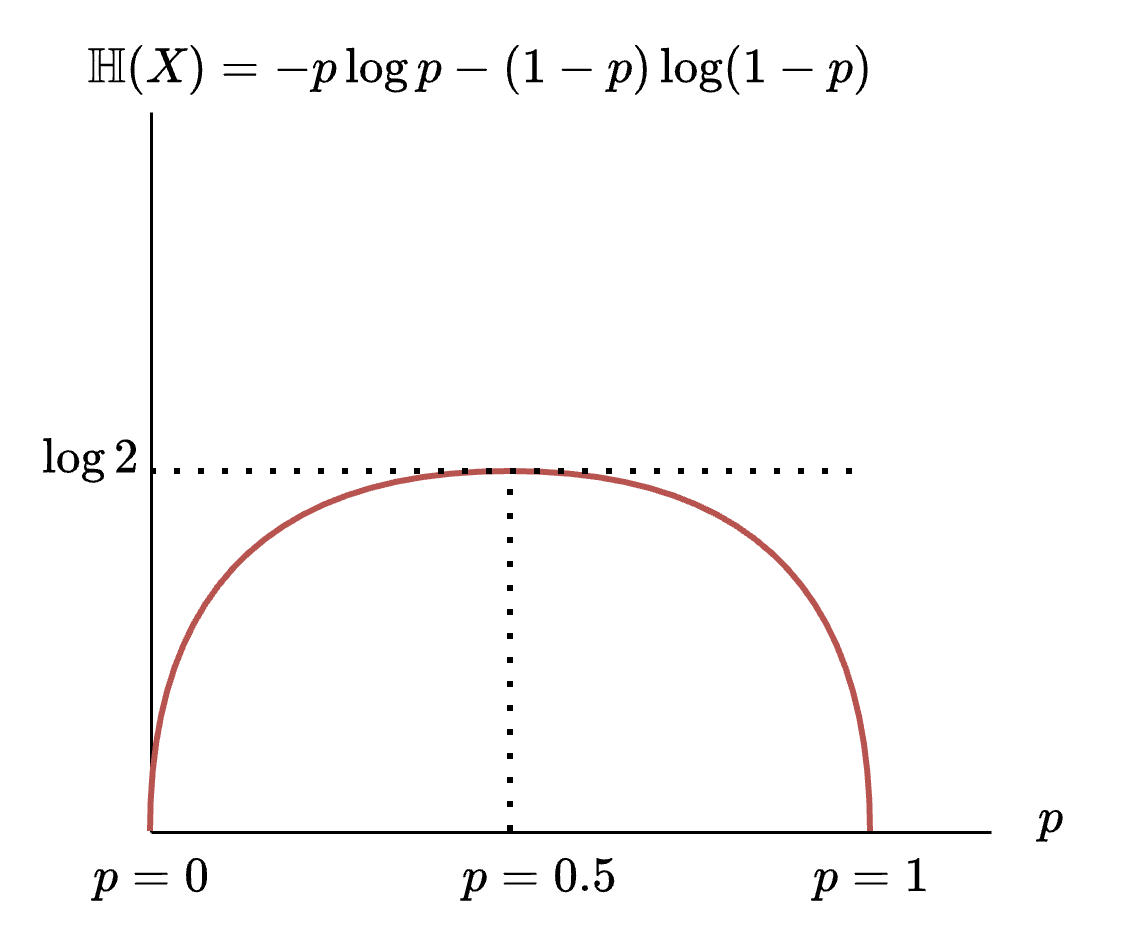
\includegraphics[width=0.5\linewidth]{Figures/entropy.png}
    \caption{Illustration of the entropy of a coin toss as $p$, the probability of getting heads, varies between $0$ and $1$. At both $p=0$ and $p=1$, one of the two outcomes is certain to happen. Thus, we can determine the outcome of the coin toss with $100\%$ accuracy, and so observing the outcome of the toss would give us no additional information in these two cases. If the probabilities are equal, $p = 1-p = 0.5$, entropy is maximized.}
    \label{fig:entropy_cointoss}
\end{figure}

\subsection{Estimating $p(z|\mathcal{D};\theta)$}\label{section:estimating_p|z}

Remember that running inference (equation \ref{eq:inference}) is hard; this is because it requires us to know $p(z|\mathcal{D};\theta)$. As a result, we need to resort to approximating $p(z|\mathcal{D};\theta)$ with some ``guess'' $q_\nu (z)$ such that $q_\nu (z) \approx p(z|\mathcal{D};\theta)$. We can vary $\nu$, the \textbf{variational parameters} in order to improve our approximation. To do this, we want to \textbf{maximize} the similarity between our trial distribution, $q_\nu (z)$, and our target distribution, $p(z|\mathcal{D};\theta)$.

But \textbf{how} do we quantify the \textbf{similarity between two distributions}?

\subsubsection{Don't Fear the Theta}
In the following, we will see me write many probability distributions with explicit reference to the fact that they are deduced from the model parameters, i.e.\ you will see a lot of things like $P(~\cdot~;\theta)$. You can largely ignore this if you'd prefer; many notes do. However, omitting the $\theta$ makes it easy to forget how to actually calculate and/or estimate these distributions. So I have maintained the presence of the $\theta$ below.

\subsubsection{KL Divergence}\label{section:kl_divergence}

We can use a measure called the \textbf{Kullback-Leibler (KL) Divergence} to quantify the similarity between two distributions. The definition of (forward\footnote{We'll cover the difference between the \textbf{forward} and \textbf{reverse} KL divergences in just a moment.}) KL divergence is:
\begin{equation}\label{eqn:kl_divergence_cont}
    D_\text{KL}(p||q) = \int \text{d}x ~ p(x) ~\log\frac{p(x)}{q(x)}  = \mathbb{E}_{x \sim p(x)} \left[\log \frac{p(x)}{q(x)} \right] 
\end{equation}

For the case of discrete variables where $P(x)$ and $Q(x)$ are \textbf{probability mass functions}, we would write the KL divergence as:
\begin{equation}\label{eq:kl_divergence_discrete}
    D_\text{KL}(p||q) = \sum_{x} p(x) \log \left[ \frac{p(x)}{q(x)}\right]
\end{equation}

Note that the KL divergence is strictly \textbf{non-negative}. We can see this by invoking \textbf{Jensen's Inequality} for \textbf{convex} functions, which states that $\mathbb{E}[f(x)] \geq f(\mathbb{E}[X])$ (see Appendix \ref{appendix:jensen}). We first rewrite the KL divergence as:
\begin{equation}\label{eq:KL_signs}
    D_\text{KL}(p||q) = -\mathbb{E}_{x \sim p(x)} \left[\log \frac{q(x)}{p(x)} \right] \geq -\log \mathbb{E}_{x \sim p(x)}\left[\frac{q(x)}{p(x)} \right]
\end{equation}
We have flipped the sign in order to invert the fraction in the argument. A $\log$ is \textbf{concave}, and therefore  a $-\log$ is \textbf{convex}, hence the sign of the inequality. We then expand the argument of the logarithm using the definition of what an expectation value is to obtain:
\begin{align}
    D_\text{KL}(p||q) \geq - \log \int \text{d}x~ p(x) \frac{q(x)}{p(x)} 
    &= - \log \int \text{d}x~q(x)\\
    &= - \log 1 \\
    &= 0
\end{align}
Thus $D_\text{KL}(p||q) \geq 0$, \textit{Q.E.D}.

We imagine $p(x)$ to be some ``true'' distribution, which we are trying to model with $q(x)$. Note the immediate similarity to the \textbf{Shannon entropy} which we discussed last subsection. 

KL divergence is also a measure of \textbf{surprisal}: how ``surprised'' would we be (remember, this denotes how much ``information'' would we gain) if we were to find out that the true distribution is $p(x)$, given that we've been modeling it as $q(x)$? We can equally think of KL divergence as a measure of how ``wrong'' we were when we used $q(x)$; the more wrong we were, the more we'd be surprised. Ideally, we want to be surprised as little as possible; in other words, we want our model to have been doing a good job all along even before $p(x)$ was revealed to us\footnote{Of course, in reality, $p(x)$ is never ``revealed'' to us-- if it were, why would we be trying to model it!}.

In the same way that the Shannon entropy can encode the number of \textbf{bits} required to convey information of an outcome, the KL divergence is interpreted as the \textbf{extra number of bits} required to encode data drawn from $P(x)$ if the encoding scheme was designed for $Q(x)$ \cite{haase2017information} (see Appendix \ref{appendix:kl_divergence_bits}).

\subsubsection{Forward and Reverse KL} \label{section:f_and_r_kl}
This section is indebted to the work presented in ref.~\cite{Ganguly2021}.

KL divergence is \textbf{not symmetric} in its arguments, i.e.\ 
\begin{equation}\label{eq:forwards_KL_neq_backwards_KL}
    D_\text{KL}(p||q) \ne D_\text{KL}(q||p)
\end{equation}
which means that it is not a \textbf{metric} (see Appendix \ref{appendix:KL_metric}). 

Let's take a closer look at what happens when $p(x)$ and $q(x)$ vary with respect to each other for the \textbf{forwards} KL divergence:

\begin{equation}\label{eq:forwards_kl}
    D_\text{KL}(p||q) = \int \text{d}x~ p(x)\log\left[\frac{p(x)}{q(x)}\right]
\end{equation}

We observe the following trends for the \textbf{forward KL divergence}:

\begin{itemize}
    \item If $q(x)\rightarrow 0$, the KL divergence is \textbf{large}. Thus, in the forwards KL, $q(x)$ is \textbf{zero avoiding} and will \textbf{overestimate} $p(x)$.
    \item If $q(x)$ is small where $p(x)$ is large, then we are heavily penalized; the forward KL divergence is \textbf{large} in this case.
    \item If $q(x)$ is large where $p(x)$ is small, we actually get away with this; the forward KL divergence is \textbf{small}. Each point in the integrand is ``weighted'' by $p(x)$, so if $p(x)$ is small, the integrand is small, even if $q(x)$ is large\footnote{Remember that polynomials always ``beat'' logarithms, e.g.\ $x^{-1} \log(x)\rightarrow 0$ as $x\rightarrow \infty$. You can check this yourself by Taylor expanding $\log(x)$ and see what happens when you multiply it by $x^{-1}$.}.
    \item If $q(x) \rightarrow p(x)$, then KL divergence is \textbf{small}, as the argument of the logarithm approaches $1$. This is what we expect, and is the whole point of using the KL divergence as the objective.
\end{itemize}

The \textbf{reverse} KL divergence is, of course,
\begin{equation}\label{eq:backwards_kl}
    D_\text{KL}(q||p) = \int \text{d}x~ q(x)\log\left[\frac{q(x)}{p(x)}\right]
\end{equation}

and the inverse of the arguments above apply, i.e.\ reverse KL divergence \textbf{underestimates} $p(x)$, and we are penalized when $q(x)$ is large at points where $p(x)$ is small.

\subsubsection{Using KL Divergence to Approximate $q_\nu (z)$}

Now, we want to approximate $p_\theta(z|\mathcal{D})$ with $q_\nu(z)$. Therefore, we are interested in computing:
\begin{equation}
    D_\text{KL}(q_\nu(z) || p(z|\mathcal{D}; \theta)) = \int \text{d}z ~ q_\nu(z) ~\log \frac{q_\nu(z)}{p(z|\mathcal{D};\theta)} = \mathbb{E}_{z \sim q_\nu (z)} \left[\log \frac{q_\nu (z)}{p(z|\mathcal{D}; \theta)} \right]
\end{equation}
and where we have kept $\theta$ in the argument to explicitly denote that $p(z|\mathcal{D};\theta)$ is a function of the model parameters. 

$p(z|\mathcal{D} ;\theta)$ is a function of the model because the \textbf{latent variables} are determined by the model. In the MoG case, for example (figure \ref{fig:mixture-of-gaussians}), each datapoint will be assigned to one of the Gaussians; this assignment is given by some label, $k$, which is a latent variable. This assignment can only be determined by the model itself (via its parameters), and hence $P(z|\mathcal{D})$ is parametrized by $\theta$.

Using the properties of logarithms, and by writing $p(z|\mathcal{D};\theta) = p(z, \mathcal{D} ;\theta)/p(\mathcal{D};\theta) = p(z, \mathcal{D} ;\theta)/p(\mathcal{D};\theta)$, we obtain:

\begin{align}
    D_\text{KL}(q_\nu(z) || p(z|\mathcal{D};\theta)) = &\int \text{d}z~q_\nu(z)\left[\log~q_\nu(z) - \log~p(z, \mathcal{D};\theta) + \log~p(\mathcal{D};\theta) \right] \\
    = &~~ \log~p(\mathcal{D};\theta) + \int \text{d}z~q_\nu(z)\left[\log~q_\nu(z) - \log~p(z, \mathcal{D};\theta) \right]
\end{align}
with the final equality following from the fact that $P(\mathcal{D})$ is independent of $z$. We use the definition $\mathbb{E}_{x\sim p(x)}[\phi] = \int \text{d}x ~ p(x) \phi(x)$ for a general function $\phi$ of some random variable $x\sim P(x)$ to rewrite the integral:

\begin{equation}\label{eq:kl_no_log}
    D_\text{KL}(q_\nu(z) || p_\theta(z|\mathcal{D})) = \log~p_\theta(\mathcal{D}) + \mathbb{E}_{z \sim q_\nu(z)}\left[\log~q_\nu(z) - \log~p_\theta(z, \mathcal{D}) \right]
\end{equation}

We immediately run into the problem that we \textbf{cannot calculate KL divergence directly}. This is because we can see that evaluation of the KL divergence still requires us to calculate $p(z|\mathcal{D};\theta)$, which we are specifically trying to avoid computing! Therefore, we will try to seek out some sort of bound on this quantity.

\subsubsection{Evidence Lower Bound (ELBO)}

We trivially rearrange equation \ref{eq:kl_no_log} (note the change of signs in the $\mathbb{E}$ term as we move it to the left hand side) to obtain:
\begin{equation}
    \mathbb{E}_{z\sim{q_\nu(z)}}\left[\log~p(z, \mathcal{D};\theta) - \log~q_\nu (z) \right] = \log~p(\mathcal{D};\theta) - D_\text{KL}(q_\nu (z) ||p(z|\mathcal{D};\theta)) = \text{ELBO}(q_\nu, \theta)
\end{equation}
and we denote this as the \textbf{E}vidence \textbf{L}ower \textbf{Bo}und (ELBO).

And we can now see that this quantity is something to \textbf{maximize}, as we want to minimize the KL divergence, which now appears on the right hand side with a negative sign. We now invoke Jensen's Inequality, which relates $f(\mathbb{E}[x])$ to $\mathbb{E}[f(x)]$ for a random variable, $x$, and some function $f$ (see Appendix \ref{appendix:jensen}). This inequality gives us (for a \textbf{concave} function):
\begin{equation}\label{eq:ELBO}
    \text{ELBO}(q_\nu, \theta) 
    = 
    \mathbb{E}_{z \sim q_\nu (z)}\left[\log\frac{p(z, \mathcal{D};\theta)}{q_\nu (z)}\right] 
    \leq 
    \log~\mathbb{E}_{z \sim q_\nu (z)}~\left[\frac{p(z, \mathcal{D};\theta)}{q_\nu (z)}\right]
\end{equation}

We rewrite 
\begin{equation}
    p(z, \mathcal{D};\theta) = \prod_{i=1}^N p(x^{(i)}, z^{(i)};\theta)
\end{equation}
where the index $i \in [1, N]$ runs over our dataset, $\mathcal{D}$, of length $N$. We then use the fact that $\mathbb{E}_{z \sim q_\nu (z)}\left[f(x)\cdot g(z)\right] = f(x)\cdot\mathbb{E}_{z \sim q_\nu (z)} \left[g(z)\right]$ to rewrite equation \ref{eq:ELBO} as

\begin{equation}\label{eq:ELBO_i}
    \text{ELBO}(q_\nu, \theta) 
    = 
    \sum_{i=1}^N \text{ELBO}_i(x^{(i)}, q^i_\nu(z^{(i)});\theta)
    =
    \sum_{i=1}^N\mathbb{E}_{z \sim q_\nu (z)}\left[\log\frac{p(x^{(i)}, z^{(i)};\theta)}{q^i_\nu (z^{(i)})}\right] 
\end{equation}
and we have defined $\text{ELBO} = \sum_i \text{ELBO}_i$. Note that we have now explicitly given $q$ a superscript $i$ for each data point $x^{(i)}$. This is as each $x^{(i)}$ has its own value for the latent variable, $z^{(i)}$; in the MoG case, different values of $z^{(i)}$ mean that the examples are drawn from different Gaussians, each of which is expressed by a different normal distribution: $P(x^{(i)} | z^{(i)}=j) = \mathcal{N}(\mu_j, \Sigma_j) = q^{i}$.

Let's step back and consider what we've done to get here. We wanted to find a function, $p(z|\mathcal{D})$, but we quickly realized that the requirement we compute a marginal makes this function intractable. Then, we invoked something called the KL divergence, which is a measurement of similarity between two distributions. We said that if we minimized the KL divergence between $p(z|\mathcal{{D}})$ and some trial distribution, $q_\nu (z)$, whose parameters $\nu$ we are free to vary, then $q_\nu (z)$ is a good estimate for $p(z|\mathcal{D})$. We used the definition of the KL divergence to derive something which we called the ELBO, which is a quantity that we want to \textbf{maximize}, as it increases when $p(z|\mathcal{D})$ and $q_\nu (z)$ are similar. We then used Jensen's Inequality to find yet another function, which bounds our ELBO from above. This upper bound appears on the rightmost side of equation \ref{eq:ELBO}.

Why is this bound useful? Is it something we can easily calculate? If it isn't, then there's no point in introducing it as an upper bound to our ELBO, which is the thing we want to maximize. Thankfully, it is. We have:

\begin{align}
    \text{ELBO}(q_\nu, \theta) \leq \log~\mathbb{E}_{z \sim q_\nu (z)}~\left[\frac{p(z, \mathcal{D};\theta)}{q_\nu (z)}\right] &= \log \left[ \int \text{d}z~q_\nu (z) \frac{p(z, \mathcal{D};\theta)}{q_\nu (z)} \right] 
    \\
    &= \log \left[ \int \text{d}z~p(z, \mathcal{D};\theta)\right] 
    \\
    &= \log p(\mathcal{D};\theta)
\end{align}

Notice that Jensen's Inequality allowed us to move the integration (i.e.\ the $\mathbb{E}$) inside of the $\log$, which is what gets us the nice cancellation inside of the integral. This leads us to:

\begin{align}\label{eq:final_elbo}
    \text{ELBO} \leq \text{Evidence} &= \log p(\mathcal{D} ;\theta)\\ 
    &= \log \prod_{i=1}^{N} p(x^{(i)};\theta)
    \\    
    &= \sum_{i=1}^{N}\log p(x^{(i)}; \theta)
    \\
    &= \sum_{i=1}^N \log \sum_{z^{(i)}} p(x^{(i)}, z^{(i)} ;\theta)\\
    &= \ell(\theta)
\end{align}

Therefore, the ELBO gives us a calculable lower bound on the log likelihood of the data, $\ell(\theta)$, also known as the log of the \textbf{evidence}. 

How does this relate to our original goal of minimizing KL divergence? Some further rearrangement gives:

\begin{equation}
    D_\text{KL}(q_\nu(z)||p(z | \mathcal{D};\theta)) \geq 0 \Rightarrow \log p (\mathcal{D} ;\theta) - \text{ELBO} \geq 0
\end{equation}

and we can trivially see that increasing the ELBO will decrease the KL divergence. 

Remember that the log likelihood, $\ell(\theta)$, is something that we can no longer calculate directly due to its dependence on the values of latent variables (see Equation \ref{eq:final_elbo}), which we cannot \textbf{observe} directly. However, we have just derived the ELBO something which we \textbf{can} calculate, and which gives us a method of producing a lower-bound estimate on the likelihood. 

In the next Section \ref{section:expectation_maximization}, we will take a look at the expectation maximization (EM) algorithm. It allows us to estimate the value of the log likelihood for a current choice of model parameters, $\theta^t$, and how to iteratively update our choices of the parameters, $\theta^{t}\rightarrow \theta^{t+1}$, to maximize $\ell(\theta)$ even though we can't calculate it directly.

\subsection{Expectation Maximization (EM) Algorithm}\label{section:expectation_maximization}

We now turn to a demonstration of how to use the ELBO in order to update our model parameters given some \textbf{unlabelled} dataset, $\mathcal{D}= \{x^{(i)}\}_{i=1}^N$.

During unsupervised learning, we optimize machine learning models with some parameters, $\theta$, by \textbf{maximizing likelihood}. We define \textbf{log likelihood} as follows:
\begin{equation}\label{eq:maximum_likelihood}
    \ell(\theta) = \log \prod_{i=1}^N p(x^{(i)}; \theta) = \sum_{i=1}^N \log p(x^{(i)}; \theta)
\end{equation}

However, we have seen before that our model may also be described by some \textbf{latent variables}, $z^{(i)}$, i.e.\
\begin{equation}
    \ell (\theta) = \sum_{i=1}^N \log p(x^{(i)}; \theta) = \sum_{i=1}^N \log \sum_{z^{(i)}} p(x^{(i)}, z^{(i)} ;\theta)
\end{equation}
where we have $p(x^{(i)}, z^{(i)};\theta) = p(x^{(i)}|z^{(i)})p(z^{(i)})$. 

Once again, $z^{(i)}$ could be, for example, the label of which Gaussian our example belongs to in the Mixture of Gaussians (MoG) model (recall Figure \ref{fig:mixture-of-gaussians}). In this case, $z^{(i)}$ is described by some \textbf{multinomial} distribution, $z \sim \text{Multinomial}(\phi)$ where $P(z=j) = \phi_{j}$ and clearly $\sum_j \phi_j =1$. We know that $z^{(i)}$ is the label denoting which Gaussian the $i\text{th}$ data point belongs to, and hence $x | z=j \sim \mathcal{N}(\mu_j, \Sigma_j)$ where $\mu_j$ and $\Sigma_j$ are the mean and covariance matrix parameterizing the $j\text{th}$ Gaussian in our mixture.

Another example (taken from ref.~\cite{Chuong2008}) would be a case where we are given the outcomes of coin tosses from two biased coins, $A$ and $B$, and we are asked to estimate the probability of getting \textbf{heads} from each of the two coins. We can denote these probabilities with $\theta_A$ and $\theta_B$. How would we go about estimating these $\theta$'s if we don't know which coin toss performed on which coin?

The problem we now encounter in these cases is that we \textbf{don't know the values of the latent variables for each example}, and as such we cannot maximize equation \ref{eq:maximum_likelihood} directly. In the MoG case, we are trying to model some complicated probability density using a sum of Gaussians, but we don't know which Gaussian each individual data point, $x^{(i)}$, belongs to (see Figure \ref{fig:which_gaussian}).

\begin{figure}
    \centering
    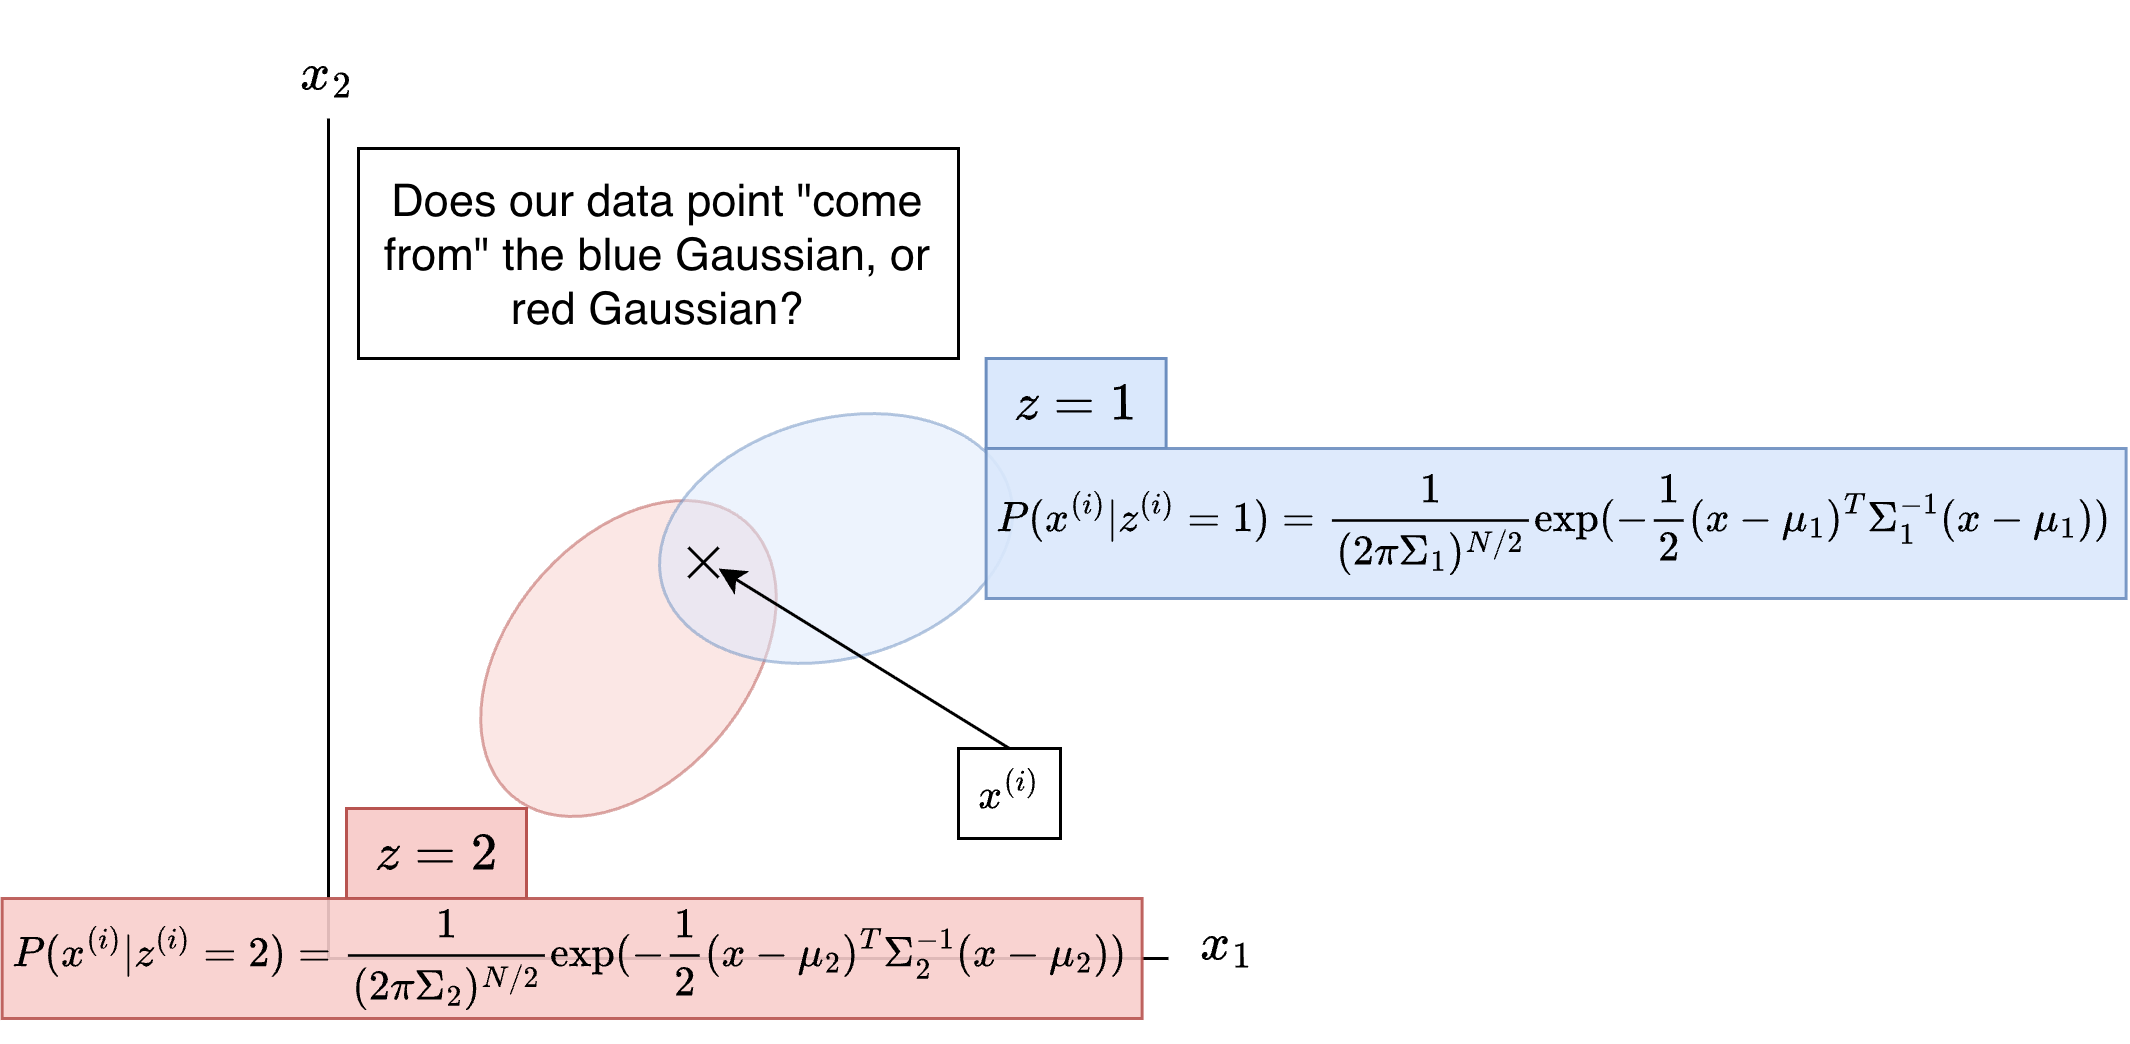
\includegraphics[width=0.85\linewidth]{Figures/which_gaussian.png}
    \caption{Example where we have some Mixture of Gaussians model. Say we observe some given data point, $x^{(i)}$, denoted as a black cross on this diagram. How are we to know which of our two Gaussians this data point ``belongs'' to, i.e.\ what is the value of its latent variable, $z^{(i)}$? All we can do is calculate the probability it comes from either Gaussian 1 (blue) or Gaussian 2 (red), and adjust our parameters $\Sigma$ and $\mu$ for each Gaussian to best match the data. To get this ``best match'', we select parameters giving the \textbf{maximum likelihood} of the data.}
    \label{fig:which_gaussian}
\end{figure}

We now turn to the landmark algorithm proposed by Dempster, Laird, and Rubin \cite{Dempster1977}. We begin by motivating the use of such an algorithm. In this algorithm, we iteratively improve our model by \textbf{guessing the values of the latent variables} for each example, and then updating our model parameters based on those guesses.

We try to illustrate this in Figure \ref{fig:em_algorithm_mog}. We take a look at our data, and try to guess the latent variables for each example. Then, we update $\theta$ such that the \textbf{likelihood} of the observed data is \textbf{maximized} for our guess of latent variables. 

\begin{figure}
    \centering
    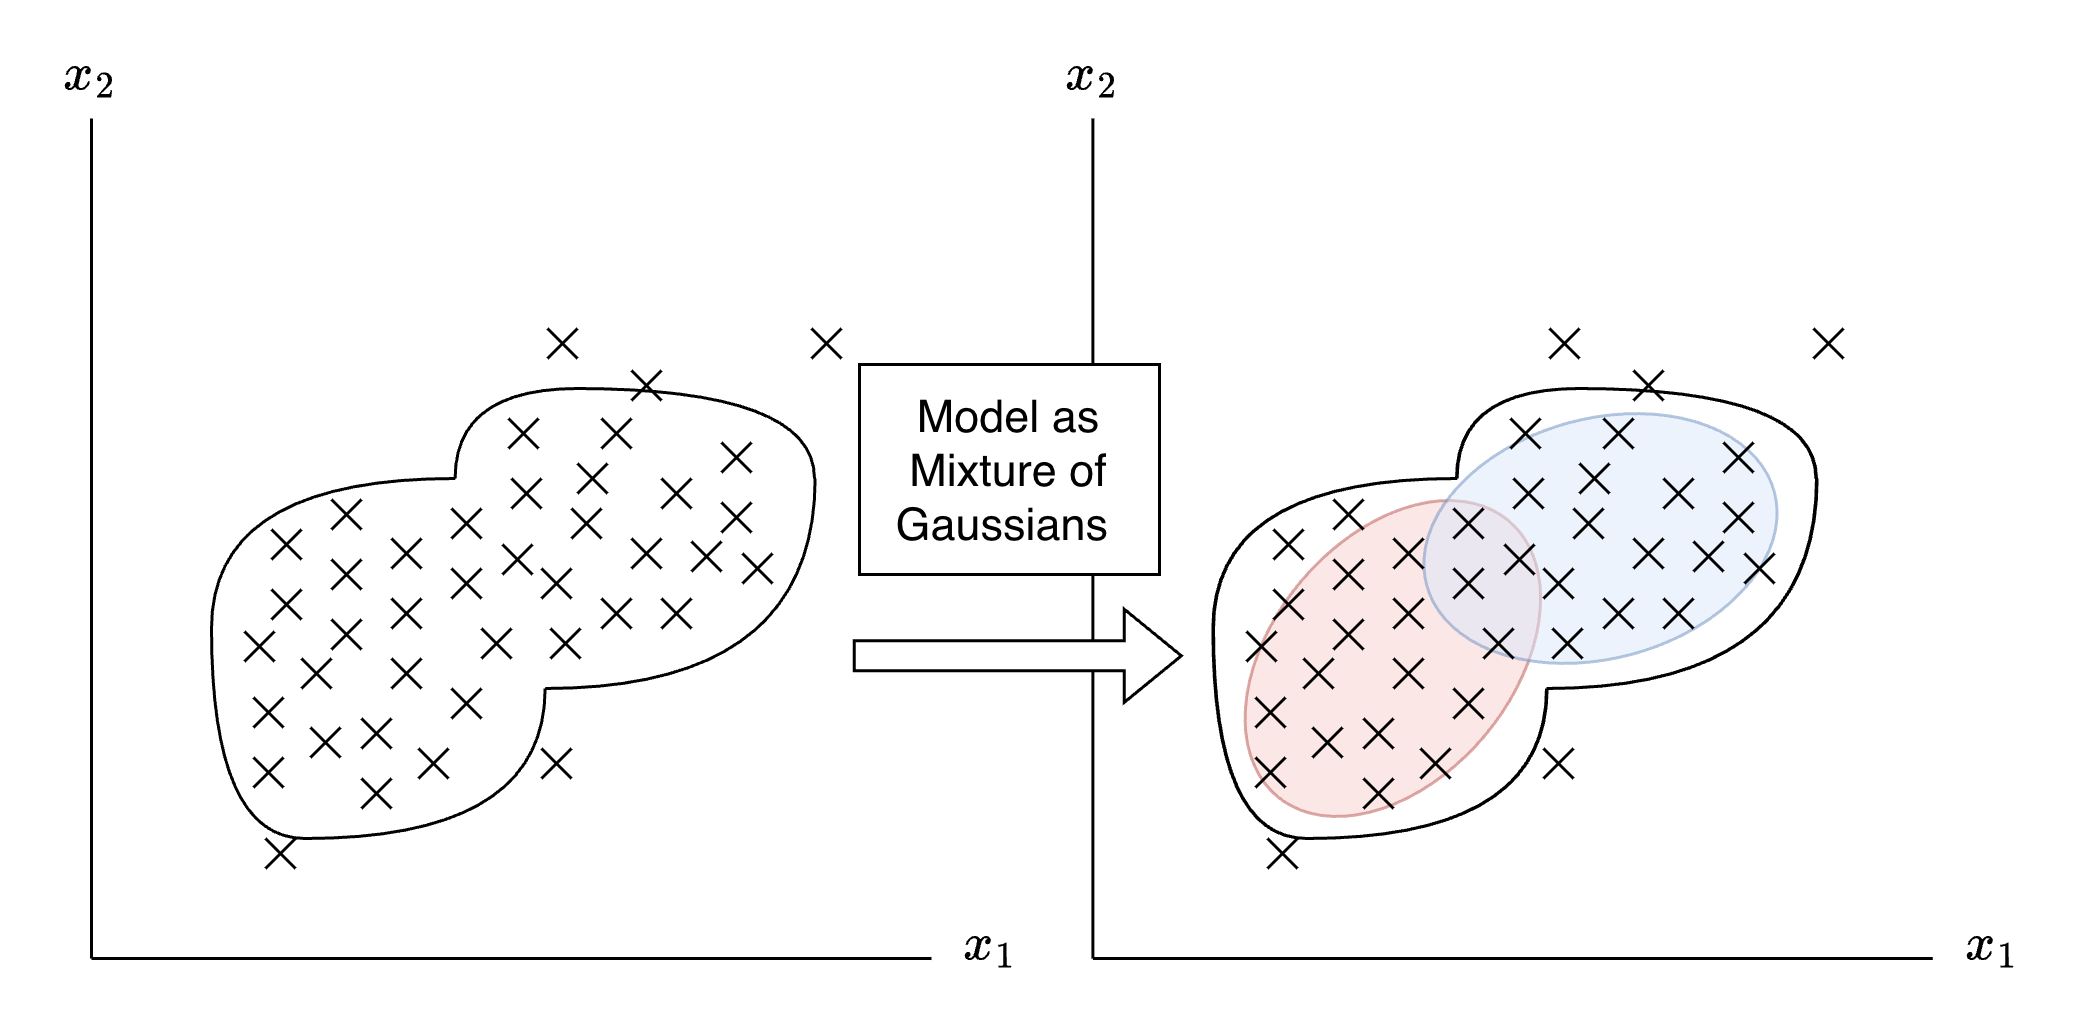
\includegraphics[width=0.85\linewidth]{Figures/mog.png}
    \caption{Fake dataset which we imagine modelling as a mixture of two Gaussians, denoted as red and blue.}
    \label{fig:em_algorithm_mog}
\end{figure}

\subsubsection{Graphical Interpretation of the EM Algorithm}
We turn to Figure \ref{fig:em_graphical} to demonstrate what the expectation maximization algorithm is doing. For each ``guess'' of the latent variables, we first calculate the likelihood of the data given these guesses. We can call this the ``guessed'' likelihood function, represented by the green line. Then, we modify our model parameters to move to the maximum point on this line. We can see from our graph that we would like our ``guessed'' likelihood to be equal to the ``true'' likelihood for our current values of $\theta$; this way, we have the tightest possible lower bound on the true likelihood function, and formulate our \textbf{estimate} (E-Step) of the underlying likelihood. Thus, we would like the inequality in equation \ref{eq:ELBO_i} to be an equality. This is true if the argument is \textbf{constant}:

\begin{equation}\label{eq:arg_is_const}
    \frac{p(x^{(i)}, z^{(i)};\theta)}{q_\nu^{(i)}(z^{(i)})} = \text{const.}
\end{equation}

i.e.\ is a random variable which always takes the same value with certainty. We denote the probability distribution for such a random variable $x$ with $p(x=\mathbb{E}[x]) = 1$ (see Appendix \ref{appendix:jensen}). Note that $q^{(i)}$ has been given a superscript to denote that the precise form of $q$ differs for each example; in the MoG case, this is because different $x^{(i)}$'s will be drawn from different Gaussians, $x^{(i)}|z^{(i)} \sim \mathcal{N}({\mu_{z^{(i)}}}, \Sigma_{z^{(i)}})$, with $q^i = p(x^{(i)}|z = z^{(i)})$.

Therefore, we choose

\begin{equation}\label{eq:q_choice}
    q^{(i)}(z^{(i)}=j; \theta)= \frac{p(x^{(i)}, z^{(i)}=j ;\theta)}{\sum_{l=1}^k p(x^{(i)}, z^{(i)}=l;\theta)}~, ~z^{(i)} \in [1, k]
\end{equation}
where the requirement given by Equation \ref{eq:arg_is_const} means the $\nu$ now must given by some of our model's parameters $\theta$, which in the MoG case are our $\mu_j$'s and $\Sigma_j$'s for the different Gaussians. Therefore, we remove the $\nu$ subscript and explicitly show that $q^{(i)}$ is parametrized by $\theta$. We explicitly denote that the latent variable $z^{(i)}$ has $k$ possible values. If we have a MoG model with 3 Gaussians, $k=3$.

We will now introduce some notation to explicitly denote that we are iterating over our estimates for the posterior, $q \approx P(z|\mathcal{D} ;\theta)$, and our model parameters, $\theta$, with time. Therefore, we shall write $q^{(i), ~t}$ and $\theta^{t}$ to denote our approximations for the posterior and model parameters, respectively, at time $t$.

This choice of $q^i$ now means that the inequality between evidence at the ELBO (Equation \ref{eq:final_elbo}) is an \textbf{equality}, i.e.

\begin{equation}\label{eq:elbo_equality}
    \ell(\theta^{t}) = \sum_{i=1}^N \text{ELBO}_i(x^{(i)}, q^{(i),t~}(z^{(i)});\theta^t)
\end{equation}

We know that for an arbitrary next choice of model parameters, $\theta^{t+1}$ that Equation \ref{eq:elbo_equality} bounds the likelihood from below, i.e.
\begin{equation}\label{eq:maximize}
    \ell(\theta^{t+1}) \geq \sum_{i=1}^N \text{ELBO}_i(x^{(i)}, q^{(i), t~}(z^{(i)});\theta^{t+1})    
\end{equation}
and we adjust $\theta$ for fixed $q^t$ to maximize the right-hand side; this is the \textbf{m-step} (maximization).

\begin{figure}
    \centering
    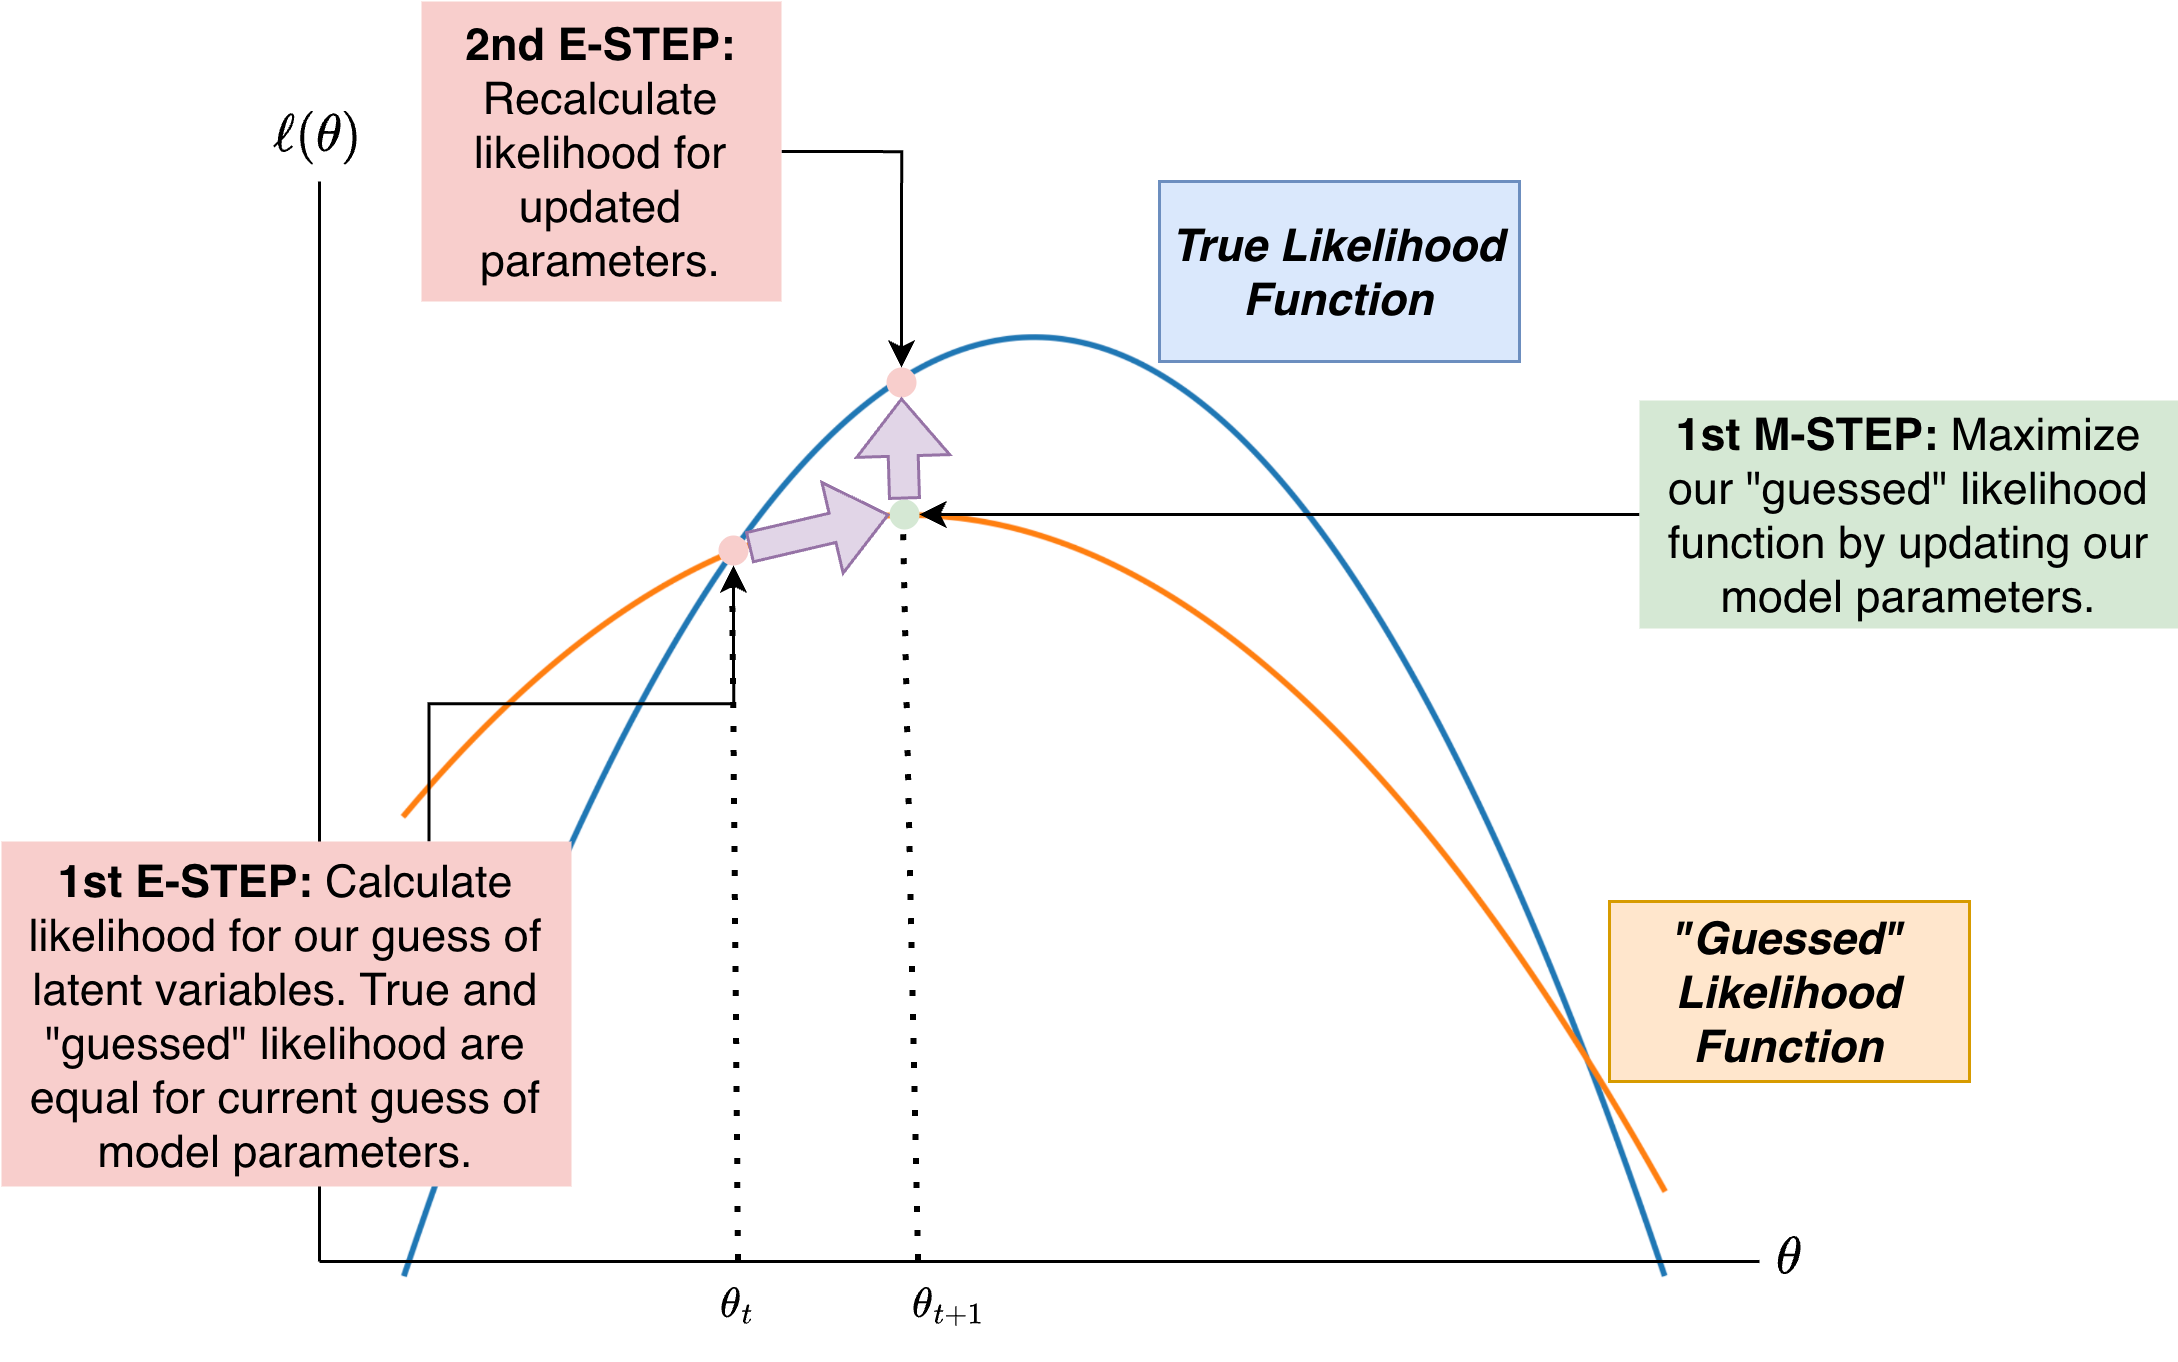
\includegraphics[width=0.75\linewidth]{Figures/em_graphical.png}
    \caption{Graphical demonstration of the E and M steps for the EM algorithm. We calculate our $q$ using equation \ref{eq:q_choice}. We know that, for this choice of $q$, our estimated likelihood (orange curve) is equal to the true likelihood (blue curve), but we can't calculate the latter directly. We move to the maximum of the orange curve during our M step by updating our model parameters from $\theta_t$ to $\theta_{t+1}$}
    \label{fig:em_graphical}
\end{figure}

\begin{em_box}
Repeat for $t=1, 2....$ until convergence.
\begin{itemize}
    \item (1) \textbf{E-Step (Expectation)} Calculate $q^{(i), t~}(z^{(i)}=j; \theta^t)~~ \forall~~(i, j)$ for current timestep $t$ using Equation \ref{eq:q_choice}. Use this to calculate likelihood, $\ell(\theta^t)$ as in equation \ref{eq:elbo_equality}.
    \item (2) \textbf{M-Step (Maximization)} Update model parameters $\theta^t \rightarrow \theta^{t+1}$ to maximize our estimate for the likelihood, as in equation \ref{eq:maximize}.
\end{itemize}
\end{em_box}



\printbibliography

\newpage
\appendix
\section{Jensen's Inequality}\label{appendix:jensen}

Jensen's Inequality provides us with a method of relating $\mathbb{E}[f(x)]$ to $f(\mathbb{E}[x])$ for some function, $f$, and some random variable, $x$. There's no reason we'd expect these two properties to be exactly equal! 

Let's say that we have a probability distribution defined as follows: our random variable, $x$, can take two values: $x = \{x_1, x_2 \}$, each with probability $0.5$. Therefore: $$P(x=x_1) = P(x=x_2) = 0.5$$ and hence $\mathbb{E}[x] = (x_1+ x_2)/2$, which is of course the midpoint between the values. We can then draw a \textbf{chord} between $f(x_1)$ and $f(x_2)$, as we have done on Figure \ref{fig:jensen}. The \textbf{midpoint} of this chord is the \textbf{expected value} of the function. We can see that, in the \textbf{concave} case (Figure \ref{fig:jensen}), this midpoint appears below the curve at $\mathbb{E}[x]$. This is opposite to the \textbf{convex} case. 

In which situation does Jensen's Inequality become an equality? We could trivially have the case where $f(x)$ is a flat line; however, in this case, $f(x)$ is not strictly concave, and we are interested in probability distributions (concave things).  In order to have a strictly \textbf{concave} (or \textbf{convex}) function where $f(\mathbb{E}[x]) = \mathbb{E}[f(x)]$, we would need the random variable, $x$, to be constant. More formally, we would have $p(x = \mathbb{E}[x]) = 1$, i.e. $p(x) = \delta(x-\mathbb{E}[x])$ where we have introduced the \textbf{Dirac delta function}, $\delta$, which is a generalized function that is 0 everywhere except $\mathbb{E}[x]$, and which integrates to 1 when the integration range includes the point $\mathbb{E}[x]$. We illustrate this case in Figure \ref{fig:jensen_equality}.

\begin{figure}[!h]
    \centering
    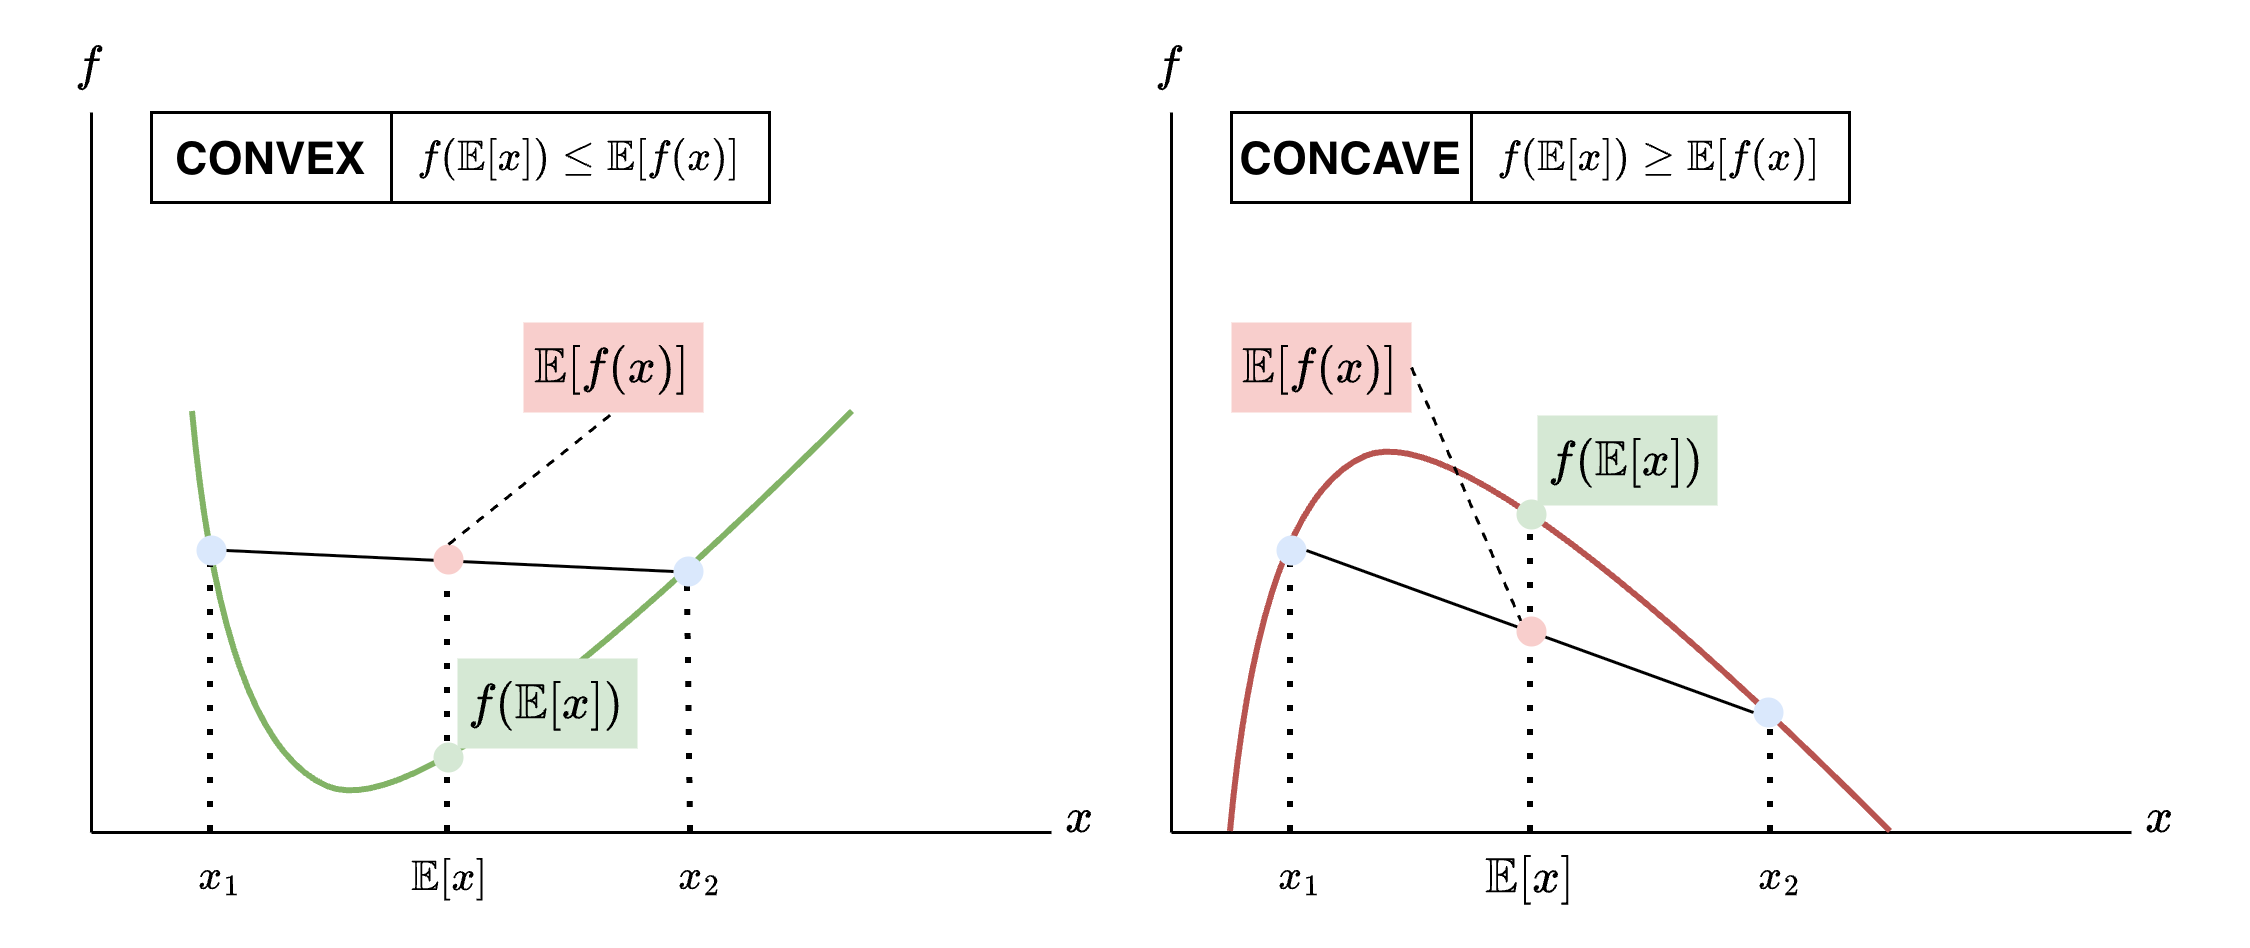
\includegraphics[width=0.85\linewidth]{Figures/convex_and_concave.png}
    \caption{Illustration of Jensen's Inequality for both a \textbf{convex} and a \textbf{concave} function (i.e.\ something which could be a probability density function).}
    \label{fig:jensen}
\end{figure}



\begin{figure}[!h]
    \centering
    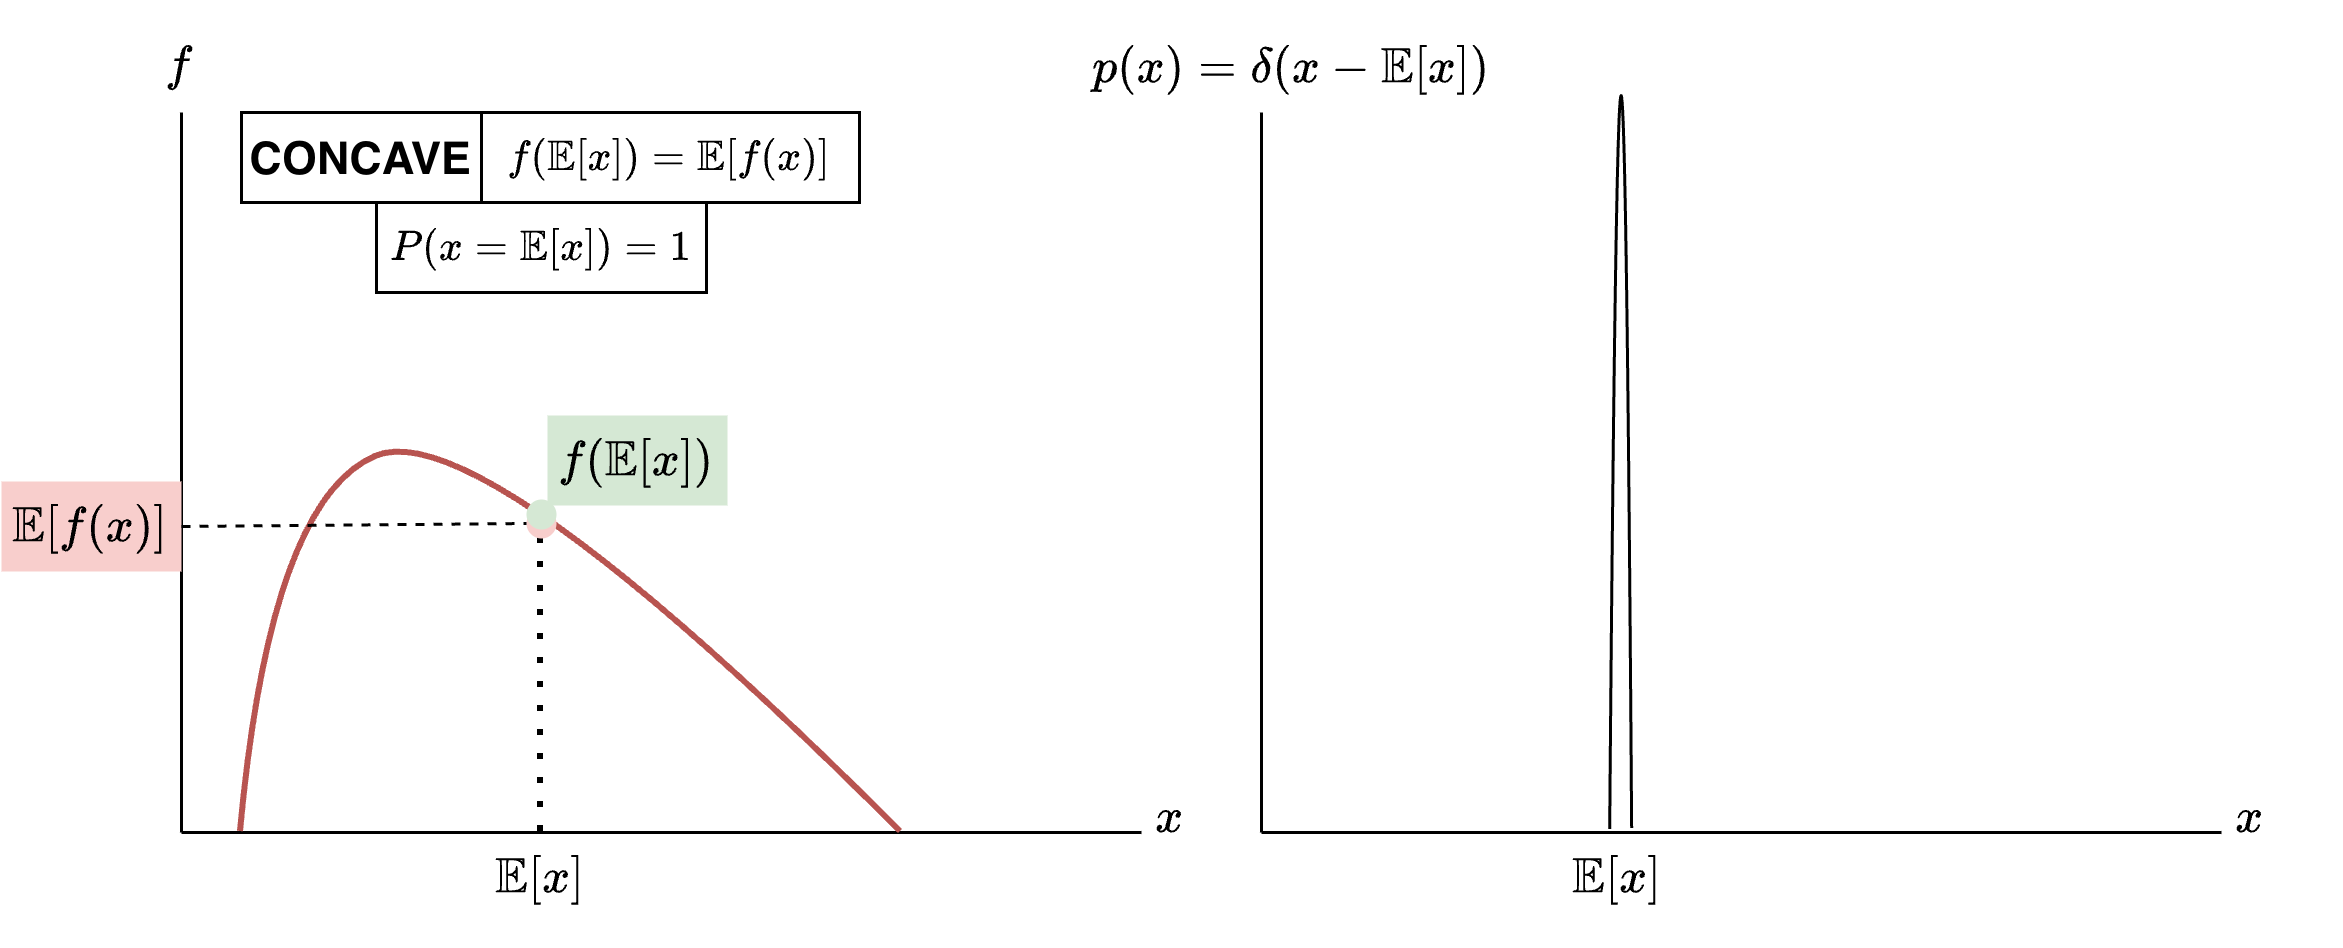
\includegraphics[width=0.9\linewidth]{Figures/jensen_equality.png}
    \caption{Case where Jensen's Inequality becomes an equality for some concave function, $f(x)$; here, we have $x=\text{const.}$, i.e.\ it is a random variable which always takes the value of $\mathbb{E}[x]$ with probability 1.}
    \label{fig:jensen_equality}
\end{figure}

\clearpage
\section{KL Divergence, Expanded}

\subsection{KL Divergence is Not a Metric}\label{appendix:KL_metric}

An example of a metric for measuring the distance between two points in some vector space where $\{\textbf{x}_1, \textbf{x}_2\} \in \mathbb{R}^n$ would be the \textbf{norm},  $|\textbf{x}_1-\textbf{x}_2|$. 

Clearly, the norm is \textbf{symmetric in its arguments}, meaning $|\textbf{x}_1-\textbf{x}_2| = |\textbf{x}_2-\textbf{x}_1|$. This is a necessary, but not sufficient, condition for a function to be a \textbf{metric}. We summarize the conditions of a \textbf{metric}, and whether the KL Divergence satisfies each of these requirements, in Table \ref{tab:is_kl_metric}.

We know from the definition of the KL Divergence in Section \ref{section:kl_divergence}, as well as our discussion of forward and reverse KL Divergence in \ref{section:f_and_r_kl} in that we actually obtain different estimates, $q(x)$, for our true underlying distribution, $p(x)$, depending on whether we use $D_{\text{KL}}(p||q)$ or $D_{\text{KL}}(q||p)$. Therefore, KL Divergence fails to satisfy the \textbf{symmetry} requirement.

We have additionally shown that the KL Divergence is non-negative in Section \ref{section:kl_divergence}, satisfying the \textbf{non-negativity} requirement. 

And there are plenty of counterexamples that prove the KL Divergence doesn't meet the requirement of the \textbf{triangle inequality} $D_\text{KL}(p||q) \nleq D_\text{KL}(p||r) + D_\text{KL}(r||q)$.

We know that the KL Divergence must satisfy the \textbf{identity} requirement if the first argument is non-zero due to the presence of the $\log \frac{p(x)}{q(x)}$, which is 0 if $p(x) = q(x)$. Note that it's possible for $p$ to be 0 everywhere, making $D_{\text{KL}} = 0$ even if $p\neq q$. Strictly, we can only assume that the forwards and reverse KL Divergences fulfill the identity requirement if $p$ and $q$ are not zero everywhere. In these notes, we have been exclusively assuming that $p$ and $q$ are some real and modelled probability density functions, respectively, and hence have to integrate to 1. This prevents them from being 0 everywhere.

\begin{table}[!h]
    \centering
    \begin{tabular}{ll}
\hline
\textbf{Condition}                                    & \textbf{Satisfied by KL Divergence?} \\ \hline
SYMMETRY: $d(x, y) = d(y, x)$                         & No                                   \\
NON-NEGATIVITY: $d(x, y) \geq 0$                      & Yes                                  \\
TRIANGLE INEQUALITY: $d(x, z) \leq d(x, y) + d(y, z)$ & No                                   \\
IDENTITY: $d(x, y) = 0 \leftrightarrow x = y$         & Yes                                  \\ \hline
\end{tabular}
    \caption{Summary of the conditions required for a function to be a metric \cite{Hunter_RealAnalysis_Ch13}, and which of these conditions are met by the KL Divergence.}
    \label{tab:is_kl_metric}
\end{table}

\subsection{KL Divergence as Measurement of ``Extra Bits''}\label{appendix:kl_divergence_bits}

KL Divergence can be seen as representing the number of bits required to encode $p(x)$ if we are modelling it using our trial distribution, $q(x)$ \cite{haase2017information}. This is a direct and obvious extension to our concept of \textbf{surprisal}; we expect to require zero extra bits to encode $p(x)$ if we were modeling it perfectly with $q(x)$, i.e.\ $q(x)=p(x)$. \textbf{Zero surprise} means we need \textbf{zero extra bits}.

To see this, let's revisit some information theory and unpack the KL Divergence a bit more carefully. We can start by expanding the log:

\begin{align}\label{eq:KL_div_expanded}
    D_\text{KL}(P||Q) = \sum_x P(x) \log \frac{P(x)}{Q(x)} 
    &= \sum_x P(x)\log P(x) &&- \sum_x P(x) \log Q(x) 
    \\
    &= -\mathbb{H}(P) &&+ \mathbb{H}(P, Q)
\end{align}
where we now introduce the \textbf{cross-entropy} $\mathbb{H}(P, Q)$ between the two distributions, $P$ and $Q$. 

Let's examine a simple example where there are two outcomes, 0 or 1. Say that $P(x=1) = 1$, i.e. $x=1$ with certainty. What if we get things wrong and we are modeling $P(x)$ with some distribution $Q(x)$ where we have $Q(x=0)=Q(x=1)=0.5$? 

We know from Section \ref{section:entropy_and_information} that the entropy of $P(x)$ will be 0 if it predicts one of its events with certainty. Therefore, $\mathbb{H}(P) = 0$. We can now calculate the \textbf{cross-entropy}, $\mathbb{H}(P, Q)$ as follows:

\begin{equation}
    \mathbb{H}(P, Q) \text{[nats]} = -0\times\log(0.5) -1 \times \log(0.5) = \log2
\end{equation}
One bit is $\log2$ nats from Equation \ref{eq:self-information}, and hence here our \textbf{cross-entropy} is 1 bit; we know that $\mathbb{H}(P)=0$ for this example, and hence the KL divergence is also 1 bit. 

Therefore, to encode the distribution $P$ with a system used to encode $Q$, we need 1 extra bit. This makes sense as our distribution $Q$ gives us an equal probability of both outcomes, when we know that in reality, one of these two outcomes occurs with certainty, i.e.\ $x=1$ every time. We can imagine that for every sample from the distribution $Q$, we need to ``tell'' the distribution $Q$ that, actually, the correct answer is 1, which is 1 bit's worth of information.

What if our model $Q(x)$ was a little better? For example, say $Q(x=1) = 0.9$? Then we have

\begin{equation}
    \mathbb{H}(P, Q) \text{[nats]} = -0 \times \log(0.1) - 1 \times \log(0.9) \approx 0.105
\end{equation}
which is \textbf{0.152 bits}. The interpretation of this is natural; $90\%$ of the time, we expect our model distribution $Q(x)$ to be correct, and therefore we need a much smaller number of bits on average encode $P(x)$.

\end{document}
